\documentclass[10pt,twoside,openright]{memoir}
\usepackage[T1]{fontenc}
\usepackage{amsmath, amsthm, amssymb}
\usepackage{amsfonts}
\usepackage{siunitx}
\usepackage{palatino}
\usepackage[version=3]{mhchem}
\usepackage{enumerate}
\usepackage{graphicx}
\usepackage[colorlinks=true, linkcolor=blue]{hyperref}
\usepackage{typedref}
\allowdisplaybreaks
\usepackage[protrusion=true,expansion=true]{microtype}
\usepackage{type1cm}
\usepackage{lettrine}
\usepackage{makeidx}
\usepackage{xspace}
\usepackage{nomencl}
%\usepackage{exsheets}
\makeindex
\makenomenclature
%This is rather a pain: Use the following command line syntax to get the nomenclature page:
%makeindex EngineeringQM_v20130303.nlo -s nomencl.ist -o EngineeringQM_v20130303.nls

\newtheorem{theorem}{Theorem}{Theorems}[section]
\newtheorem{lemma}{Lemma}{Lemmas}[section]
\newtheorem{corollary}{Corollary}{Corollaries}[section]
\newtheorem{definition}{Definition}{Definitions}[section]

\theoremstyle{definition}
\newtheorem{exercise}{Exercise}{Exercises}[section]
\newtheorem{example}{Example}{Examples}[section]

\newcommand*{\norm}[1]{\ensuremath{\left\|#1\right\|}\xspace}

\checkandfixthelayout

% See the ``Memoir customise'' template for some common customisations
% Don't forget to read the Memoir manual: memman.pdf

%\chapterstyle{companion}
\chapterstyle{veelo}


\makeatletter
\def\maketitle{%
  \null
  \thispagestyle{empty}%
  \vfill
  \begin{center}\leavevmode
    \normalfont
    {\LARGE\raggedleft \@author\par}%
    \hrulefill\par
    {\huge\raggedright \@title\par}%
    \vskip 1cm
%    {\Large \@date\par}%
  \end{center}%
  \vfill
  \null
  \cleardoublepage
  }
\makeatother


\author{J. Kono, N. A. Thompson \& G. D. Woods}
\title{Engineering Quantum Mechanics}
\date{\today}

\begin{document}
\maketitle
\tableofcontents

\nomenclature{$\mathbb{R}$}{The real numbers, such as $0.1$, $5$, $\pi$, and $-13.4$.}
\nomenclature{$\mathbb{C}$}{The complex numbers, such at $1+i$, $e^{i\pi/4}$, $12$, and $15.7i$.}
\nomenclature{$\mathbb{N}$}{The natural numbers, $1,2,3,\ldots$. By definition, $0$ is \emph{not} included.} 
\nomenclature{$h$}{Planck's constant, $h=\SI{4.136e-15}{\electronvolt \second}$.}
\nomenclature{$\hbar$}{Reduced Planck's constant, defined as $\frac{h}{2\pi} = \SI{6.582e-16}{\electronvolt\second}$.}
\nomenclature{$C[a,b]$}{Continuous functions defined on an interval $[a,b]\subset \mathbb{R}$.}
\nomenclature{$C^{1}[a,b]$}{Differentiable functions with continuous derivatives defined on $[a,b]\subset\mathbb{R}$.}
\nomenclature{$C^{\infty}$}{Infinitely differentiable functions.}
\nomenclature{$L^{2}(\mathbb{R})$}{Functions $f$ with $\norm{f}_{2}< \infty$.}
\nomenclature{$\norm{\, \cdot \, }$}{A generic norm form measuring the ``size'' of functions.}
\nomenclature{$\norm{\, \cdot \, }_{2}$}{$L^{2}$-norm.}
\nomenclature{$\norm{\, \cdot \, }_{\infty}$}{Maximum norm.}
\nomenclature{$\land$}{Logical \textrm{AND}.}
\nomenclature{$\in$}{``In''. $x\in \mathbb{R}$ means $x$ is a real number.} 
\nomenclature{$[\cdot,\cdot]$}{Generic Lie bracket. Any skew-symmetric, bilinear function satisfying a Jacobi identity.}
\nomenclature{$:=$}{``Defined as''.}
\nomenclature{$\dot{x}$}{First derivative of $x$ with respect to time.}
\nomenclature{$\ddot{x}$}{Second derivative of $x$ with respect to time.}
\nomenclature{$\forall$}{``For all''.}
\nomenclature{$\mathcal{O}(x^2)$}{Error of order $x^{2}$.}
\nomenclature{iff}{``If and only if''. We say ``$a$ iff $b$'' when $a$ implies $b$ and $b$ implies $a$.}

\newpage

\chapter*{Why Engineering Quantum Mechanics?}

%QM for engineers and materials scientists.
%QM for undergraduate students interested in solid state devices, lasers, and nanoscience and nanotechnology.
%Emphasis on nanoelectronics and nanophotonics, spintronics, and quantum computing, rather than relativistic QM, quantum field theory, and elementary particles.
%{\em Materials}: semiconductors (bulk, quantum confined, magnetic) and carbon nanotubes. 
%{\em Devices}: diodes, transistors, light emitters, photodetectors, modulators, � etc.

This book is for engineers and materials scientists interested in learning quantum mechanics. 
Though many readers will read this book out of intrinsic interest in the subject, others will do so out of necessity:
They will find their colleagues interpreting data,  diagnosing problems with instruments, or designing better devices using quantum mechanics, and they will recognize that making incremental improvements on existing technologies requires use of more precise theories. 
Perhaps there was a time when engineers and materials scientists were better off investing their time in other areas of study, such as learning to use Newtonian mechanics in increasingly complicated situations, or learning how to apply classical electrodynamics to complicated objects, but we argue that this time is over.  
There seems to be no technical field that quantum mechanics has not invaded.
In this chapter, let us look at three important sub-disciplines of engineering that are behind modern information technology --- electronics, photonics, and materials --- to observe how quantum mechanics has changed, and is changing, our world in a fundamental manner.

\section*{Electronics}

%\subsection{Miniaturization of Electronic Devices}\index{electronic devices}
\subsubsection{Need for Quantum Technologies}\index{quantum technologies}  
Moore's law: number of transistors per chip doubles every 18 months.  Has been sustained for the past 5 decades.  One way to look at Moore's law is to examine the typical feature size as a function of time.  If the current trend persists, a typical feature size will approach the size of an atom by 2060.  By $\sim$2060 the basic memory components of a computer will be the size of individual atoms.  The classical laws will have to be replaced by the laws of quantum physics--statistical, fuzzy.  Clearly, miniaturization of electronic devices is approaching a physical limit.

%\subsection{Need for Quantum Technologies}\index{quantum technologies}  
``Quantum physics holds the key to the further advance of computing in the postsilicon era.'' -- J. Birnbaum and R. S. Williams.  ``Coherent spin packets may offer genuine quantum devices through their wave-like properties.'' -- D. D. Awschalom.  Novel quantum technologies being sought $\rightarrow$ better performance and new functionality and multi-functionality

%\subsection{Emerging Technologies for Information Processing}\index{information processing}

Use discrete, quantized degrees of freedom in a physical device to perform information processing functions.

\subsection{Spintronics}\index{spintronics}  Use spins in solid state devices.  Improve information processing.
 Add new functionalities.
  Quantum Spin Electronics
Tunneling/transport of quantum confined spin states
Spin dependent resonant tunneling devices and spin filtering
Spin FETs (�spin gating�)
Spin LEDs, electroluminescent devices, and spin lasers
Coherent Spin Electronics
Optically generated coherent spin states and coherent control of propagating spin information - optical encoders and decoders
Quantum Information Processing
Qubits using coherent spin states a|0> + b|1>, a2 + b2 = 1
Spin based quantum computing, teleportation, code breaking and cryptography.
Realization of Spin-Based Devices
technical issues:
How strongly can one create carriers of a given spin?
How long can one sustain the spin polarization?
How can one modulate or control the spin?
How sensitively can one detect the spin?



\subsection{Quantum Computation and Communications}\index{quantum computation}\index{quantum communication} Devise and implement quantum-coherent strategies for computation and communication.
Reinvention of computer science and information theory in a way that is consistent with quantum physics.
Take just a few minutes to break all the secret codes used by the world�s security agencies
Totally secure communication by encoding information in photons of light
�Teleportation� of quantum states of matter across large distances
Can generate true random numbers
Two States:
A qubit = a state in a 2D Hilbert space
Quantum Mechanical Superposition:
Quantum computation consists of preparation, operation, and measurement.
Toward Solid-State Realization of QIP
The race is on!
Intensive search for realistic approaches to building a quantum computer
Solid-state systems offer a much greater degree of control over design and fabrication, necessary for constructing large-scale devices.
Coherent states are very easily damaged by uncontrolled interactions with the environment � decoherence
Unavoidable decoherence will cause the quantum information to decay ? main obstacle
Decoherence causes a collapse of the superposition state into a single eigenstate ? loss of parallelism


\section*{Photonics}\index{photonics}
In light-emitting diodes, solar cells, and optical communications, one uses optoelectronic devices --- devices that generate, manipulate, and detect light.
Inside such optoelectronics is quantum engineering.
Electronic states in heterostructures can be engineered using quantum mechanics.
Quantum Engineering of Electronic Structure ---> Tailored Electronic and Optical Properties.
Various types of quantum confinement are possible with semiconductor heterostructures. The Quantum Cascade Laser.
Light can be confined as well.
Light can be confined and guided.
A photonic circuit.  Future: Silicon-Based Integrated Optoelectronic Circuits.


\section*{Materials}

\subsection{Nanomaterials}\index{nanomaterials}  \ce{C60}, carbon nanotubes, graphene, nanoshells, ...

 introduction to electrical conduction in solids; metals and insulators; hydrogen atom; periodic table; molecules; from bonds to bands; Pauli�s exclusion principle; particle in a box; and quantum wells, wires, and dots.

%%%%%%%%%
%%%%%%%%%

\chapter{Entering the Quantum World}

Materials properties (electrical, optical, magnetic, mechanical) w/o quantum mechanics.
Quantum concepts and methods $\rightarrow$ applications to atoms, molecules, and solids.
Band theory of solids $\rightarrow$ metals, semiconductors, and insulators.
The de Broglie hypothesis and derivation of the time-independent Schr\"{o}dinger equation.

\begin{itemize}
%   
\item   What makes solids different from atoms and molecules?
\item What are the differences between a metal and an insulator (or a semiconductor)?
\item When is quantum mechanics important (when does classical physics fail)?
\item How can one determine the dimensionality (D) of a system?
\item What physical quantity best distinguishes 0D, 1D, 2D, and 3D systems?
%
\end{itemize}   



\section{Breakdown of Classical Physics}

\subsection{Classical electrical conduction (the Drude model)}   

We treat an electron as a classical particle with mass $m$ = 9.11 $\times$ 10$^{-31}$~kg and charge $-e$ = $-$1.6 $\times$ 10$^{-19}$~C.  Newton's equation of motion is written as
%%%
\begin{align}
F = ma,
\end{align}
%
where $F$ (N) is the force acted on the electron and 
\begin{align}
a = {dv \over dt} = {d^2 x \over d^2 t}
\end{align}
%
is the acceleration (m/s$^2$).  We solve this equation to obtain a trajectory $x = x(t)$, or $\vec{r}(t) = (x(t),y(t),z(t))$ and $\vec{F} = m\vec{a}$ in 3D.

We apply a DC voltage, $V$ (V), to a conductor of length $L$ (m) and cross section $A$ (m$^2$).  The electric field $E$ (V/m) is
%
\begin{align}
E = {V \over L}
\label{E-field}
\end{align}
%
The force on the electron is $F = -eE$ (N).  Then the equation of motion is
%
\begin{align}
F = -eE = ma = m {dv \over dt},
\label{EOM}
\end{align}
%
where $v$ (m/s) is the velocity.  The solution to Eq.~\eqref{EOM} is
%
\begin{align}
v(t) = - {eE \over m}t + v_0.
\end{align}
%
We introduce the scattering time, $\tau$ (s), as the average time between scattering events (by phonons and defects).  Then
%
\begin{align}
v_{avg} = - {eE \over m} \tau.
\end{align}
%
If the electron density is $N_e$ (m$^{-3}$), the current density, $J$ (C/s$\cdot$m$^2$), is then
%
\begin{align}
J = - N_e e v_{avg} = {e^2 N_e \tau \over m} E = \sigma_0 E,
\label{current-density}
\end{align}
%
where
%
\begin{align}
\sigma_0 = e N_e \mu_e
\label{conductivity}
\end{align}
%
is the (DC) conductivity (1/$\Omega \cdot$m) and
%
\begin{align}
\mu = {e \tau \over m}
\label{mobility}
\end{align}
%
is the electron mobility.

The conductivity is related to the (DC) resistivity, $\rho_0$ ($\Omega \cdot$m), through
%
\begin{align}
\sigma_0  = {1 \over \rho_0},
\end{align}
%
and the resistance, $R$ ($\Omega$), is
%
\begin{align}
R = \rho_0 {L \over A},
\label{resistance}
\end{align}
%
while the current (A)
%
\begin{align}
I = J A.
\label{current}
\end{align}
%
Using Eqs.~\eqref{E-field}, \eqref{current-density}, \eqref{resistance}, and \eqref{current}, we get Ohm's law
%
\begin{align}
V = I R.
\label{current}
\end{align}
%

\subsection{The Hall effect}

Equation \eqref{conductivity} indicates that the conductivity is determined by both the density and mobility.  One can separately determine the density and mobility if one measures the Hall effect in addition to the conductivity.

In a Hall effect experiment, one applies a magnetic field, $B$ (T), perpendicular to the current, $I$.  There will be a Lorentz force in the direction perpendicular to both $B$ and $I$, because of which electrons accumulate on one side of the sample, producing an electric field, $E_H$, which is called the Hall field.  In equilibrium, the Lorentz force and the force due to the Hall field will balance:
%
\begin{align}
-e B v_{avg} = -e E_H.
\label{Hall-balance}
\end{align}
%
Combining Eqs.~\eqref{current-density} and \eqref{Hall-balance}, we obtain
%
\begin{align}
E_H = R_H J B,
\label{Hall-balance}
\end{align}
%
where
%
\begin{align}
R_H = - {1 \over N_e e}
\label{Hall-coef}
\end{align}
%
is the Hall coefficient (m$^3$/C).

\section{Wave-Particle Duality}

Planck's relation for photons:

\begin{align}
E = h \nu
\end{align}

Einstein's relativity:



\begin{align}
E^2 = c^2 p^2 + m^2_0 c^4
\end{align}


\section{Time-Independent Schr\"{o}dinger's Wave Equation}\index{Schr\"odinger equation!time-independent}



\section{Quantum Confinement}\index{quantum confinement}

Let us consider a two-dimensional sample with size $L \times L$ (m$^2$).
%
\begin{align}
- {\hbar^2 \over 2m} \nabla^2 \psi(x,y) = - {\hbar^2 \over 2m} \left ({\partial^2 \over \partial x^2} + {\partial^2 \over \partial y^2} \right) \psi(x,y) = E \psi(x,y)
\end{align}
%
\begin{align}
- {\hbar^2 \over 2m} \left ({1 \over X(x)} {\partial^2 X \over \partial x^2} + {1 \over Y(y)} {\partial^2 Y \over \partial y^2} \right) = E
\end{align}
%
  Quantum box with infinite barrier height.  Energy quantization.

%\section{Bound States in Quantum Wells}\index{bound states!quantum well}
   %Normalization.  Orthonormality.  Parity.  Zero-point energy.  Finite-barrier quantum wells.  \ce{GaAs}/\ce{AlGaAs} quantum wells.

\section{Expectation Value}\index{expectation value}

The probabilistic interpretation of the wave function, $\psi(x)$, is such that
%
\begin{align}
|\psi(x)|^2 = P(x)
\end{align}
%
is the probability density.  Namely, the probability of finding the particle at position between $x$ and $x + dx$ is given by $|\psi(x)|^2dx$.  Therefore, the wave function has to be normalized in the following sense:
%
\begin{align}
\int^{\infty}_{-\infty} |\psi(x)|^2 dx = 1.
\end{align}
%
Similarly, in three dimensions, the probability of finding the particle in an infinitesimally small region, $dxdydz$, is given by $|\psi(x,y,z)|^2dxdydz$, and the normalization requirement is
%
\begin{align}
\int^{\infty}_{-\infty} \int^{\infty}_{-\infty}  \int^{\infty}_{-\infty}  |\psi(x,y,z)|^2 dxdydz = 1.
\end{align}
%
In the following, we will discuss only the one-dimensional case without loss of generality.

Given the wave function, $\psi(x)$, the most likely position can be calculated.  This is called the expectation value of $x$ and given by
%
\begin{align}
\left <x \right > = \int^{\infty}_{-\infty} x P(x) dx = \int^{\infty}_{-\infty} \psi^*(x) x \psi(x) dx,
\end{align}
%
which is the weighted average.

The momentum $p_x$ (= $\hbar k_x$) and $x$ are canonically conjugate.  The wavefunction can also be described in $k$-space (momentum space), as opposed to real ($x$-) space.  The wavefunction $\psi(k_x)$ has the same probabilistic interpretation as $\psi(x)$, but it is not expressed in terms of momentum.  The probability that the particle has a momentum value between $\hbar k_x$ and $\hbar (k_x + dk_x)$ is given by $|\psi(k_x)|^2dk_x$.  The wavefunction has to be normalized as
%
\begin{align}
\int^{\infty}_{-\infty} |\psi(k_x)|^2 dk_x = 1.
\end{align}
%
Given the wave function, $\psi(k_x)$, the expectation value of momentum $p_x$ is calculated as
%
\begin{align}
\left <p_x \right > = \hbar \int^{\infty}_{-\infty} \psi^*(k_x) k_x \psi(k_x) dk_x.
\label{expected-mom}
\end{align}
%

Real space and $k$-space are connected through Fourier transformation:
%
\begin{align}
\psi(k_x) &= \frac{1}{\sqrt{2\pi}} \int^{\infty}_{-\infty} \psi(x) e^{-ik_x x} dx \label{FT-1}\\
\psi(x) &= \frac{1}{\sqrt{2\pi}} \int^{\infty}_{-\infty} \psi(k_x) e^{ik_x x} dk_x \label{FT-2}
\end{align}
%
By taking the complex conjugate of Eq.~\eqref{FT-1}, we obtain
%
\begin{align}
\psi^*(k_x) = \frac{1}{\sqrt{2\pi}} \int^{\infty}_{-\infty} \psi^*(x) e^{ik_x x} dx .
\label{FT-3}
\end{align}
Also, by performing the integral on the right hand side of Eq.~\eqref{FT-1} by parts, we obtain
%
\begin{align}
\psi(k_x) = -\frac{i}{\sqrt{2\pi}} \frac{1}{k_x} \int^{\infty}_{-\infty} \frac{\partial \psi(x)}{\partial x} e^{-ik_x x} dx .
\label{FT-4}
\end{align}
%
Furthermore, by substituting Eqs.~\eqref{FT-3} and \eqref{FT-4} into Eq.~\eqref{expected-mom}, we rewrite the expectation value of momentum as
%
\begin{align}
\left< p_x \right > &= -i\hbar \int^{\infty}_{-\infty} dx' \int^{\infty}_{-\infty}  dx \, \psi^*(x') \, \frac{\partial\psi(x)}{\partial x} \, \frac{1}{2\pi} \int^{\infty}_{-\infty} dk_x e^{-ik_x(x-x')}\\
  &= \int^{\infty}_{-\infty} \psi^*(x) \left [ -i\hbar \frac{\partial}{\partial x}\right ] \psi(x) dx\\
  &= \int^{\infty}_{-\infty} \psi^*(x) \hat{p}_x \psi(x) dx \label{expected-mom-2},
  \end{align}
%
where we introduced the momentum operator
%
\begin{align}
\hat{p}_x := -i\hbar \frac{\partial}{\partial x}
\label{momentum-op}
\end{align}
%
and used
%
\begin{align}
\delta(x-x') = \frac{1}{2\pi} \int^{\infty}_{-\infty} dk_x e^{-ik_x(x-x')},
\end{align}
%
where $\delta(x)$ is the Dirac delta function.

Equation \eqref{expected-mom-2} can be extended to calculate the expectation value of any observable, $A$: 
%
\begin{align}
\left< A \right > = \int^{\infty}_{-\infty} \psi^*(x) \hat{A} \psi(x) dx
\label{expected-A}
\end{align}
%
where $\hat{A}$ is the operator associated with $A$.  For example, for the kinetic energy, $T$, the corresponding operator is defined as
%
\begin{align}
\hat{T} := \frac{\hat{p}^2_x}{2m} = - \frac{\hbar^2}{2m} \frac{\partial^2}{\partial x^2},
\label{kinetic-energy}
\end{align}
% 
and the expectation value is given by
%
\begin{align}
\left< T \right > = \int^{\infty}_{-\infty} \psi^*(x) \hat{T} \psi(x) dx = \int^{\infty}_{-\infty} \psi^*(x) \left [ - \frac{\hbar^2}{2m} \frac{\partial^2}{\partial x^2} \right ] \psi(x) dx .
\label{expected-kin-eng}
\end{align}
%
Note that the position $x$ is a number, as opposed to an operator, in real space, i.e., $\hat{x}$ = $x$.  Thus, any function of $x$, such as the potential energy $V(x)$ is a number also, and its expectation value can be calculated as
%
\begin{align}
\left< V \right > = \int^{\infty}_{-\infty} \psi^*(x) \hat{V}(\hat{x}) \psi(x) dx = \int^{\infty}_{-\infty} \psi^*(x) V(x) \psi(x) dx .
\label{expected-pot-eng}
\end{align}

\section{Time-Dependent Schr\"{o}dinger's Wave Equation}\index{Schr\"odinger equation!time-dependent}
%
Let us consider the Schr\"{o}dinger equation for a free particle in one dimension, for which $V(x)$ = 0:
%
%
\begin{align}
-\frac{\hbar^2}{2m} \frac{d^2 \psi(x)}{dx^2} = E \psi(x).
\label{SE-free-ptcle}
\end{align}
%
The general solution to this equation can be written as
%
\begin{align}
\psi(x) = A e^{ik_xx} + B e^{-ik_xx},
\label{free-particle-solution-1}
\end{align}
%
where the wave number $k_x$ is related to the energy $E$ as
%
\begin{align}
k_x = \frac{\sqrt{2mE}}{\hbar}
\label{wn-free-ptcle}
\end{align}
%
and $A$ and $B$ are constants.  From Eq.~\eqref{free-particle-solution-1} we see that
%
\begin{align}
\hat{p}_x\psi(x) = (\hbar k_x) A e^{ik_xx} + (-\hbar k_x) B e^{-ik_xx},
%\label{wn-free-ptcle}
\end{align}
%
which suggests that the first (second) term represents a free-particle state that is traveling with momentum $\hbar k_x$ ($-\hbar k_x$).  

In analogy to the classical theory of traveling plane waves, we introduce the time dependence as
%
\begin{align}
\Psi(x,t) &= A e^{i(k_xx - \omega t)} + B e^{-i(k_xx - \omega t)}\\
&= (A e^{ik_xx} + B e^{-ik_xx})e^{-i\omega t},
\label{wf-free-ptcle}
\end{align}
%
where the temporal angular frequency. $\omega$, and spatial angular frequency (or wave number), $k_x$, are related through the dispersion relation or the energy-momentum relation:
%
\begin{align}
E = \hbar \omega = \frac{\hbar^2 k^2_x}{2m}.
\label{free-ptcle-dispersion}
\end{align}
%
Equation \eqref{wf-free-ptcle} makes it clearer that the first (second) term represents a free-particle state traveling to the right (left).  Furthermore, this wavefunction suggests the association of $k_x$ and $\omega$ with the following operators:
%
\begin{align}
\hat{k}_x &:= -i\frac{\partial}{\partial x} \label{k-op}\\
\hat{\omega} &:= i\frac{\partial}{\partial t} \label{omega-op}.
\end{align}  
%
Together with these operators, the dispersion relation, Eq.~\eqref{free-ptcle-dispersion}, suggests
the time-dependent Schr\"dingier equation:
%
\begin{align}
i\hbar \frac{\partial}{\partial t} \Psi(x,t) =  - \frac{\hbar^2}{2m} \frac{\partial^2}{\partial x^2} \Psi(x,t).
\label{TDSE-free}
\end{align}
%
In the presence of a force field, $F(x,t) = \frac{\partial V(x,t)}{\partial x}$, the dispersion relation is modified to:
%
\begin{align}
E = \hbar \omega = \frac{\hbar^2 k^2_x}{2m} + V,
\label{free-ptcle-dispersion}
\end{align}
%
and thus, the energy operator (Hamiltonian operator) can be written as
%
\begin{align}
\hat{H} = \hbar \hat{\omega} = \frac{\hbar^2 \hat{k}^2_x}{2m} + V.
\label{H-op}
\end{align}
%
Combining Eqs.~\eqref{k-op}, \eqref{omega-op}, and \eqref{H-op},  we obtain the full, time-dependent Schr\"odingier equation:
%
\begin{align}
i\hbar \frac{\partial}{\partial t} \Psi(x,t) =  \left \{ - \frac{\hbar^2}{2m} \frac{\partial^2}{\partial x^2} + V(x,t) \right \} \Psi(x,t).
\label{TDSE}
\end{align}
%


%\newpage
%\section{Separation of Variables}\index{separation-variables}
%
When the potential is stationary, i.e., $V = V(x)$, Eq.~\eqref{TDSE} can be separated into two equations describing the spatial and temporal parts, respectively.  We set $\Psi(x,y) = \psi(x) \phi(t)$, substitute it in Eq.~\eqref{TDSE}, divide both sides by $\psi\phi$, and obtain
%
\begin{align}
i\hbar \frac{1}{\phi(t)}\frac{d \phi(t)}{d t} =  - \frac{\hbar^2}{2m} \frac{1}{\psi(x)} \frac{d^2 \psi(x)}{d x^2} + V(x).
\label{TDSE-sep}
\end{align}
%
The left hand side depends only on $t$ while the right hand side depends only on $x$.  In order for this equation to hold for any values of $t$ and $x$, both sides must be equal to a constant ($E$).  Thus,
%
\begin{align}
i\hbar \frac{d \phi}{d t} &= E\phi \label{time-SE} \\
- \frac{\hbar^2}{2m} \frac{d^2 \psi}{d x^2} + V(x) &= E\psi. \label{space-SE}
\end{align}
%
Equation \eqref{time-SE} yields
%
\begin{align}
\phi(t) = A e^{-iEt/\hbar} = A e^{-i\omega t}.
\end{align}
%

This harmonically oscillating time-dependent phase factor, $e^{-i\omega t}$, always exists for a stationary state.  For example, the first three wavefunctions of the infinite-barrier square potential well can now be written
%
\begin{align*}
\Psi_1(x,t) &= \sqrt{\frac{2}{L}} \sin {\left (\frac{\pi}{L}x \right )} \cdot e^{-i\omega_1 t} \\
\Psi_2(x,t) &= \sqrt{\frac{2}{L}} \sin {\left (\frac{2\pi}{L}x \right )} \cdot e^{-i\omega_2 t} \\
\Psi_3(x,t) &= \sqrt{\frac{2}{L}} \sin {\left (\frac{3\pi}{L}x \right )} \cdot e^{-i\omega_3 t}
\end{align*}
%
where $\omega_1 = E_1/\hbar = (\hbar^2/2m) (\pi^2/L^2) /\hbar$, $\omega_2 = 4 \omega_1$, and $\omega_3 = 9\omega_1$.  This time dependence is not observable when the particle is in a single state, as can be seen by the fact that for any state $|\Psi_n(x,t)|^2 = |\psi_n(x)|^2$.  However, when the particle is in a superposition state, time-dependence does appear.  For example, when the particle is in
%
\begin{align}
\Psi = \frac{1}{\sqrt 2} (\Psi_1 + \Psi_2),
\label{superposition}
\end{align}
%
The probability density $|\Psi_n(x,t)|^2$ does oscillate as a function of time with frequency given by $\omega_2 - \omega_1$:
%
\begin{align}
|\Psi|^2 = |\psi_1|^2 + |\psi_2|^2 + 2\mathrm{Re}(\psi_1^*\psi_2) \cos(\omega_2 - \omega_1)t.
\label{interference}
\end{align}




%\newpage

%\section{Heisenberg's Uncertainty Relation}\index{uncertainty principle}

%\section{Separation of Variables}\index{separation of variables}

%%%%%%%%%%%%% CHAPTER 3 %%%%%%%%%%%%%%%%%%%%%%%%%%%%%%%%%%%%%%%%%%%%%

\chapter{Mathematical Machinery}

A regrettable amount of mathematical machinery goes into a good understanding of quantum mechanics.
This could be avoided if a good intuitive understanding of many quantum systems was possible, but as intuition is generally derived from daily experience (governed by classical laws), we cannot expect this to be the case in general. 
For this reason, we present a quick overview of the mathematical foundations of quantum mechanics in hopes that the task of learning quantum mechanics becomes \emph{easier}.
As an additional benefit, the language developed in this chapter has invaded diverse branches of engineering. 
This mathematics has proven itself especially useful in the \emph{finite element methods} that have revolutionized AutoCAD, so many engineering students will benefit from having learned this material in their quantum mechanics class. 

\section{Vector Spaces}\index{vector spaces}

Many physicists have a very good notion of what a \emph{geometric vector} is. 
For example, a particle at point $\mathbf{r}$ can be thought of as living in the \emph{vector space} $\mathbb{R}^{3}$, and two particles at point $\mathbf{r}_{1}$ and $\mathbf{r}_{2}$ can be thought of as living in the \emph{product space} $\mathbb{R}^{3}\times \mathbb{R}^{3}$, whereupon we write $(\mathbf{r}_{1}, \mathbf{r}_{2}) \in \mathbb{R}^{3}\times \mathbb{R}^{3}$. 
We know that if we have two geometric vectors $\mathbf{r}_{1}$,$\mathbf{r}_{2} \in \mathbb{R}^{3}$, we can add them together and get another vector $\mathbf{r}_{1} + \mathbf{r}_{2} \in \mathbb{R}^{3}$. And we can also \emph{stretch} a vector via $\mathbf{r} \mapsto \alpha \mathbf{r}$ whenever $\alpha \in \mathbb{R}$. 
But we can also add \emph{functions} together, and we can also stretch functions, so why don't we say functions live in a vector space, too? 
Well, many people \emph{do} say functions live in a vector space, but this vector space isn't really a \emph{geometric} vector space, as functions aren't geometric vectors, but it still behaves a lot like a geometric vector space. 
For example, if $f(x):= \sin(\theta)$, and $g(x):= \sin(2\theta)$, then $f+g$ is defined through
\begin{align*}
(f+g)(\theta):= f(\theta) +g(\theta) = \sin(\theta) + \sin(2\theta). 
\end{align*}
And if $\alpha \in \mathbb{R}$, then $\alpha f$ is defined through $\alpha f(\theta) = \alpha \sin(\theta)$.
When your vector space is filled with functions, people often call the vector space a \emph{function space}. 

\begin{example}
The space of continuous functions defined on the interval $[-1,1]$ is a function space; it is denoted by $C[-1,1]$.\index{$C[a,b]$}
\end{example}
\noindent The absolution value function $x\mapsto |x|$ is a continuous function, so it is an element of $C[-1,1]$.
\begin{example}
The space of functions having continuous first derivatives on $\mathbb{R}$ is a function space; it is denoted by $C^{1}(\mathbb{R})$.\index{$C^{1}[a,b]$}
\end{example} 
\begin{example}
The space of infinitely differentiable functions defined on $\mathbb{R}$ is a function space; it is denoted by $C^{\infty}(\mathbb{R})$.\index{$C^{\infty}(\mathbb{R})$}
\end{example}
\noindent Famous examples of $C^{\infty}(\mathbb{R})$ functions are $\sin$, $\cos$, and $\mathrm{sinc}$. The absolute value function is not $C^{\infty}(\mathbb{R})$, since it differentiates into the increasingly rambunctious $\mathrm{sgn}$-function
\begin{align*}
\mathrm{sgn}(x) := 
\begin{cases}
\phantom{-}1,	&	 x>0,	\\
\phantom{-}0,	&	x=0,	\\
-1,	&	x<0.
\end{cases}
\end{align*}
and then twice the enormously rambunctious Dirac $\delta$-function:\index{Dirac delta function}
\begin{align*}
\delta(x):= 
\begin{cases}
\infty,	&	x=0	\\
0,		&	x\ne 0.
\end{cases}
\end{align*}
Just as we like to measure the length of a geometric vector $\mathbf{r} \in \mathbb{R}^{3}$ by $|\mathbf{r}|:= \sqrt{\mathbf{r}\cdot\mathbf{r}}$, we also would like to measure the ``length'' of functions.
A function that measures the length of functions is called a \emph{norm}. 
Since we acknowledge that the ``length'' of a function is a very different thing than the length of a geometric vector, we distinguish norms from geometric lengths via giving them two bars, i.e., the norm of a function $f$ is denoted by $\norm{f}$.
\begin{example}
The \emph{maximum norm}\index{$\norm{\cdot}_{\infty}$}
\begin{align*}
\norm{f}_{\infty}:= \max_{x\in [a,b]} |f(x)|
\end{align*}
 is a norm on $C[a,b]$.
\end{example}
\begin{example}
The function
\begin{align*}
\norm{f}_{\infty, 1}:=\max\{\norm{f}_{\infty}, \norm{f'}_{\infty}\}
\end{align*}
is a norm on $C^{1}[a,b]$. 
\end{example}
\noindent The norm most important for quantum mechanics is called the $L^{2}$-norm. The $L^{2}$-norm of a function $f$ is defined as\index{$\norm{\cdot}_{2}$}
\begin{align}
\norm{f}_{2}:= \sqrt{\int_{-\infty}^{\infty} |f(x)|^{2} \, dx }.
\end{align}
This norm has a very special property: It is induced by an \emph{inner product}:\index{$\left<\cdot, \cdot\right>$}
\begin{align}\label{InnerProduct}
\left<f, g\right> := \int_{-\infty}^{\infty} f(x)^{*} g(x) \, dx.
\end{align}
Hence we can write the norm as $\norm{f}_{2}^{2} = \left<f,f\right>$. 
The function space of all functions $f$ with $\norm{f}_{2} <\infty$ is called a \emph{Hilbert space}\index{Hilbert space}. 

\begin{exercise}
Let $f(x):= \exp(-x^{2}/2)$. Compute $\norm{f}_{\infty}$, $\norm{f}_{\infty, 1}$, and $\norm{f}_{2}$.
\end{exercise}

\begin{exercise}
Let $g(x):= \mathrm{sinc}(kx)$, where $\mathrm{sinc}(\theta):= \frac{\sin(\theta)}{\theta}$. Compute $\norm{g}_{\infty}$, $\norm{g}_{\infty, 1}$, and $\norm{g}_{2}$.
\end{exercise}

\section{Linear Operators}\index{linear operator}

With the notion of a function space firmly in hand, we can define the supremely important concept of a linear operator: 
\begin{definition}[Linear Operator]\index{linear operator}
Let $\mathbb{F}$ represent $\mathbb{R}$ or $\mathbb{C}$, and let $V$ and $W$ be vector spaces. A function $\mathcal{L}\colon V \to W$ is called a \emph{linear operator} iff
\begin{align*}
\mathcal{L}[\alpha f] &= \alpha \mathcal{L}[f] & & \forall \alpha \in \mathbb{F} \land \forall f \in V, 	\\
\mathcal{L}[f+g] &= \mathcal{L}[f] + \mathcal{L}[g] & & \forall f, g\in {V}.
\end{align*}
\end{definition}
\noindent The property $\mathcal{L}[\alpha f] = \alpha \mathcal{L}[f]$ is called \emph{homogeneity}\index{linear operator!homogeneity}, and the property $\mathcal{L}[f+g] = \mathcal{L}[f] + \mathcal{L}[g]$ is called \emph{additivity}\index{linear operator!additivity}.
The most important objects in undergraduate mathematics are linear operators, though you may not recognize them as such:
\begin{example}
Differentiation is a linear operator, as 
\begin{align*}
\frac{d}{dx}(\alpha f) &= \alpha \frac{df}{dx}	\\
\frac{d}{dx}(f+g) &= \frac{df}{dx} + \frac{dg}{dx}.
\end{align*}
\end{example} 

\begin{example}
Indefinite integration is a linear operator, as
\begin{align*}
\int \alpha f(x) \, dx &= \alpha \int f(x) \, dx	\\
\int f(x) + g(x) \, dx &= \int f(x) \, dx + \int g(x) \, dx
\end{align*}
\end{example}


 \section{Operators}\index{operators}
 
An operator changes a function into another function.  In the following example, the operator $A$ changes the function $f$ into$g$:
%
\begin{align}
\hat{A}f = g
\label{operator-def}
\end{align}
%
For $\hat{A} = 1 + d/d x$, 
%
\begin{align}
g(x) = f(x) + \frac{d f}{d x}.
\end{align}
%
For $\hat{A} = \frac{d}{d x}x$, 
%
\begin{align}
g(x) = \frac{d}{d x} \left [xf(x) \right ] = f(x) + x \frac{d f}{d x} = \left ( 1 + x \frac{d}{dx} \right )f(x).
\end{align}
%
Thus, we can write the following operator equation:
%
\begin{align}
\frac{d}{d x} x =  1 + x \frac{d}{dx}.
\end{align}
%

 \section{Simple Harmonic Oscillator}\index{harmonic oscillator}
 
To become familiar with operator algebra, here we examine the problem of the one-dimensional simple harmonic oscillator (SHO).  The Hamiltonian is
%
\begin{align}
\hat{H} = -\frac{\hbar^2}{2m} \frac{d^2}{dx^2} + \frac{1}{2}m\omega^2 x^2,
\end{align}
%  
where $\omega = \sqrt{\kappa/m}$ is the characteristic frequency of the SHO, $\kappa$ is the force constant, and $m$ is the mass of the particle.  We introduce a length, $L$, in such a way that the coefficients of the two term become equal in magnitude after the change of variable through $x = L \xi$, where $\xi$ is a dimensionless coordinate.  The Hamiltonian is written in the new variable as
%
\begin{align}
\hat{H} = -\frac{\hbar^2}{2m} \frac{1}{L^2} \frac{d^2}{dx^2} + \frac{1}{2}m\omega^2 L^2 \xi^2,
\end{align}
%  
and thus, we choose $L$ such that
%
\begin{align}
\frac{\hbar^2}{2m} \frac{1}{L^2} = \frac{1}{2}m\omega^2 L^2 ,
\end{align}
%  
or, 
%
\begin{align}
L := \sqrt{\frac{\hbar}{m\omega}}.
\end{align}
%  
With this definition of $L$, the Hamiltonian is now written
%
\begin{align}
\hat{H} = \frac{\hbar \omega}{2} \left ( - \frac{d^2}{d\xi^2} + \xi^2 \right ).
\end{align}
%  

Knowing $x^2 - y^2 = (x -y)(x+y)$ for ordinary numbers, $x$ and $y$, we are tempted to write the following operator equation:
%
\begin{align}
- \frac{d^2}{d\xi^2} + \xi^2 =? \left (-\frac{d}{d\xi} + \xi \right )\left ( \frac{d}{d\xi} + \xi \right ).
\end{align}
% 
However, through simple operator algebra, one can show that
%
\begin{align}
\left (-\frac{d}{d\xi} + \xi \right ) \left ( \frac{d}{d\xi} + \xi \right )f &= - \frac{d^2f}{d\xi^2} + \xi^2f - f \label{op-rel-1}\\
 \left ( \frac{d}{d\xi} + \xi \right ) \left (-\frac{d}{d\xi} + \xi \right ) f &= - \frac{d^2f}{d\xi^2} + \xi^2f + f \label{op-rel-2}
\end{align}
% 
for an arbitrary function $f(\xi)$.  Thus, the Schr\"odinger equation can be written as
%
\begin{align}
\hat{H}\psi(\xi) = \frac{\hbar\omega}{2}\left [ \left (-\frac{d}{d\xi} + \xi \right ) \left ( \frac{d}{d\xi} + \xi \right ) + 1 \right ] \psi(\xi) = E\psi(\xi).
\end{align}
% 
We can further modify this equation into
%
\begin{align}
\left (\hat{b}^{\dagger} \hat{b} + \frac{1}{2} \right ) \psi(\xi) = \varepsilon\psi(\xi),
\end{align}
% 
where
%
\begin{align}
\hat{b}^{\dagger} &:= \frac{1}{\sqrt2} \left (-\frac{d}{d\xi} + \xi \right )  \\
\hat{b} &:= \frac{1}{\sqrt2} \left ( \frac{d}{d\xi} + \xi \right ) \label{b-def}\\
\varepsilon &:= \frac{E}{\hbar\omega}.
\end{align}
% 
Furthermore, by shifting the origin of energy through
%
\begin{align}
\varepsilon' := \varepsilon - \frac{1}{2},
\end{align}
% 
The Schr\"odingier equation simplifies to
%
\begin{align}
\hat{b}^{\dagger} \hat{b} \, \psi = \varepsilon'\psi.
\label{SHO-SE}
\end{align}
% 

By looking at Eqs.~\eqref{op-rel-1} and \eqref{op-rel-2}, one can see that the operators $\hat{b}^{\dagger}$ and $\hat{b}$ satisfy the following commutation relationship:
%
\begin{align}
[\hat{b}, \hat{b}^{\dagger}] = \hat{b} \hat{b}^{\dagger} - \hat{b}^{\dagger} \hat{b} = 1.
\label{com-rel-bb}
\end{align}
% 
By operating $\hat{b}$ on Eq.~\eqref{SHO-SE} and using Eq.~\eqref{com-rel-bb}, we can show that
%
\begin{align}
\hat{b}^{\dagger} \hat{b} \,(\hat{b}^{\dagger} \psi) = (\varepsilon' + 1)(\hat{b}^{\dagger} \psi).
\label{SHO-SE-2}
\end{align}
% 
This equation demonstrates that $\hat{b}^{\dagger}\psi$ is another eigen-solution of the Schr\"odinger equation with an eigen-energy of $\varepsilon' + 1$.  More explicitly, if $\psi_n$ is the $n$-th solution with energy $\varepsilon'_n$, $\hat{b}^{\dagger}$ makes the $(n+1)$-th state $\psi_{n+1} = \hat{b}^{\dagger}\psi_n$ with energy $\varepsilon'_{n+1} = \varepsilon'_n + 1$.  In this sense, $\hat{b}^{\dagger}$ raises the quantum index by one through the creation of one quantum ($\hbar\omega$).  Thus, $\hat{b}^{\dagger}$ is called the creation operator.  Similarly, one can show that
%
\begin{align}
\hat{b}^{\dagger} \hat{b} \,(\hat{b} \psi) = (\varepsilon' - 1)(\hat{b} \psi).
\label{SHO-SE-3}
\end{align}
% 
In this sense, $\hat{b}$ is called the annihilation operator.  Combining these two results, we can now create a ladder of states by using these operators:
%
\begin{align*}
 &. \\
 &. \\
\psi_{n+2} = \hat{b}^{\dagger}  \psi_{n+1} =  \hat{b}^{\dagger}\hat{b}^{\dagger} \psi_n, \,\, &\varepsilon'_{n+2} = \varepsilon'_{n+1} + 1 = \varepsilon'_{n} + 2 \\
\psi_{n+1} = \hat{b}^{\dagger}  \psi_{n}, \,\, &\varepsilon'_{n+1} = \varepsilon'_{n} + 1 \\
\psi_{n}, \,\, &\varepsilon'_{n} \\
\psi_{n-1} = \hat{b} \psi_{n}, \,\, &\varepsilon'_{n-1} = \varepsilon'_{n} - 1 \\
\psi_{n-2} = \hat{b}  \psi_{n-1} =  \hat{b}\hat{b} \psi_n, \,\, &\varepsilon'_{n-2} = \varepsilon'_{n-1} - 1 = \varepsilon'_{n} - 2 \\
&. \\
 &.
%\label{SHO-ladder}
\end{align*}
%
This ladder can go up to $n = +\infty$, i.e., there is no upper limit.   However, since energy has to be positive, there must be a lower limit that defines the lowest-energy state, i.e., the ground state.  We define the ground state $\psi_0$ by requiring
%
\begin{align}
\hat{b} \psi_0 = 0.
\label{SHO-GS}
\end{align}
% 
This ensures that $\varepsilon'_0 = 0$, which means that $\varepsilon_0 = \frac{1}{2}$ or $E_0 = \frac{\hbar\omega}{2}$.  By using the definition of $\hat{b}$ [Eq.~\eqref{b-def}], one write Eq.~\eqref{SHO-GS} as
%
\begin{align}
\frac{d}{d\xi} \psi_0 = -\xi \psi_0,
\label{SHO-GS-2}
\end{align}
% 
whose solution is
%
\begin{align}
\psi_0 (\xi) = A_0 \exp \left ( -\frac{\xi^2}{2} \right ),
\label{SHO-GS-wf}
\end{align}
% 
where $A_0$ is the normalization constant.  Once the ground state is known, one can obtain any state by successive operations of $\hat{b}^{\dagger}$.  For example,
%
\begin{align}
\psi_1 (\xi) &= \hat{b}^{\dagger} \psi_0 = A_1 \times 2\xi \exp \left ( -\frac{\xi^2}{2} \right ) \\
\psi_2 (\xi) &= \hat{b}^{\dagger} \psi_1 = A_2 \times (4\xi^2 -2) \exp \left ( -\frac{\xi^2}{2} \right ).
\label{SHO-ES-wf}
\end{align}
% 
The $n$-th state is written as
%
\begin{align}
\psi_n (\xi) &= (\hat{b}^{\dagger})^n \psi_0 = A_n \times H_n(\xi) \exp \left ( -\frac{\xi^2}{2} \right ),
\label{SHO-nth-wf}
\end{align}
% 
where $H_n(\xi)$ is the $n$-th Hermite polynomial.

\section{Hermitian operators}

For arbitrary, normalized functions, $\phi$ and $\psi$, one can show that the creation and annihilation operators, $\hat{b}$ and $\hat{b}^{\dagger}$, of the simple harmonic oscillator satisfy
%
\begin{align}
\int^{\infty}_{-\infty} \phi^*(\xi)\,\hat{b}\,\psi(\xi)d\xi &= \int^{\infty}_{-\infty} \phi^*\frac{1}{\sqrt2}\left(\frac{d\psi}{d\xi}+\xi\psi\right)d\xi \\
&= \frac{1}{\sqrt2}\int^{\infty}_{-\infty}\left(-\frac{d}{d\xi}+\xi\right)\phi^*\psi d\xi \\
&= \int^{\infty}_{-\infty}(\hat{b}^{\dagger}\phi)^*\psi d\xi.
\end{align}
%
In general, for a linear operator $\hat{A}$, there exists $\hat{B}$ such that
%
\begin{align}
\int \phi^* (\hat{A}\psi)d^3 \vec{r} = \int (\hat{B}\phi)^* \psi d^3 \vec{r}.
\end{align}
%
$\hat{B}$ is called the hermitian adjoint of $\hat{A}$ and denoted as $\hat{A}^{\dagger}$.  In this sense, $\hat{b}$ and $\hat{b}^{\dagger}$ are hermitian adjoints.

If a linear operator $\hat{A}$ is its own hermitian adjoint, i.e., $\hat{A} = \hat{A}^{\dagger}$, then $\hat{A}$ is said to be a hermitian operator.  In other words, if $\hat{A}$ is hermitian, then, for two arbitrary functions $\phi$ and $\psi$,
%
\begin{align}
\int \phi^* (\hat{A}\psi)d^3 \vec{r} = \int (\hat{A}\phi)^* \psi d^3 \vec{r}.
\end{align}
%
\begin{exercise}
Show that $\hat{A} = -i \frac{\partial}{\partial x}$ is hermitian.
\end{exercise}
%
\begin{exercise}
Show that $(\hat{A}^{\dagger})^{\dagger} = \hat{A}$ for any linear operator $\hat{A}$. 
\end{exercise}
%
\begin{exercise}
Show that $(\hat{A}\hat{B})^{\dagger} = \hat{B}^{\dagger}\hat{A}^{\dagger}$ for any linear operators $\hat{A}$ and $\hat{B}$. 
\end{exercise}
%
\begin{exercise}
Show that, for any linear operator $\hat{A}$, the following three operators are hermitian: $\hat{B} = \hat{A} + \hat{A}^{\dagger}$,  $\hat{C} = i(\hat{A} - \hat{A}^{\dagger})$, and $\hat{D} = \hat{A}\hat{A}^{\dagger}$.
\end{exercise}
%
\begin{exercise}
Show that $\hat{C} = \hat{A}\hat{B}$ does not have to be hermitian even when $\hat{A}$ and $\hat{B}$ are hermitian.
\end{exercise}

If $\hat{A}$ is hermitian, one can show that
%
\begin{align}
\langle A\rangle &= \int\psi^*\hat{A}\psi d^3 \vec{r} = \int(\hat{A}\psi)^*\psi d^3 \vec{r} \\
&= \int\psi (\hat{A}\psi)^*d^3 \vec{r} = \left [\int\psi^* \hat{A} \psi d^3 \vec{r}\right]^* \\
&= \langle A\rangle^*.
\end{align}
%
Hence, $\langle A \rangle$ is a real number.  An observable is a measurable dynamical variable such as the position, linear and angular momenta, kinetic energy, and total energy.  Any observable $A$ is represented by a hermitian operator $\hat{A}$ in quantum mechanics so that the expectation value $\langle A \rangle$ is a real number.
%
\begin{exercise}
Show that $\langle p_x \rangle = \langle p_x \rangle^*$.
\end{exercise}

\section{Eigenvalue Problem and Hilbert Space}
%
For any linear operator $\hat{A}$, there exist a set of numbers $\{ a_n\}$ and a set of functions $\{ u_n\}$ such that
%
\begin{align}
\hat{A}u_n(x) = a_n u_n(x),
\end{align}
%
which is called an eigenvalue equation.  The one-dimensional, time-independent Schr\"odinger equation
%
\begin{align}
\hat{H}u_n(x) = E_n u_n(x)
\end{align}
%
is a typical example of an eigenvalue equation.  In fact, the title of Schr\"odinger's original paper in 1926 was ``Quantization as an Eigenvalue Problem.''

Let us consider two eigenfunctions, $u_n$ and $u_m$, of a hermitian operator $\hat{A}$ with respective eigenvalues, $a_n$ and $a_m$, i.e., $\hat{A}u_n = a_nu_n$ and $\hat{A}u_m = a_m u_m$.  Then one can show that
%
\begin{align}
\int u_m^* \hat{A} u_n d^3 \vec{r} &= a_n \int u_m^* u_n d^3 \vec{r}, \\
\int u_n^* \hat{A} u_m d^3 \vec{r} &= a_m \int u_n^* u_m d^3 \vec{r}.
\end{align}
%
On the other hand, since $\hat{A}$ is hermitian,
%
\begin{align}
\int u_n^* \hat{A} u_m d^3 \vec{r} = \int (\hat{A}u_n)^* u_m d^3 \vec{r} = a_n^* \int u_n^* u_m d^3 \vec{r}.
\end{align}
%
Therefore,
%
\begin{align}
0 = (a_m - a_n^*) \int u_n^* u_m d^3 \vec{r}.
\end{align}
%
When $n = m$,
%
\begin{align}
0 = (a_n - a_n^*) \int |u_n|^2 d^3\vec{r}  \,\, \Rightarrow \,\,a_n = a_n^*.
\end{align}
%
Namely, the eigenvalues of a hermitian operator are real.  When $n \ne m$,
%
\begin{align}
0 = \int u_m^* u_n d^3\vec{r}.
\end{align}
%
Assuming that all $u_n$ are normalized, we can conclude that the eigenfunctions $u_n$ of a hermitian operator $\hat{A}$ are orthonormal in the sense that
%
\begin{align}
\int u_n^* (\vec{r}) u_m(\vec{r}) d^3 \vec{r} = \delta_{nm} = 
\begin{cases}
1,	&	n = m,	\\
0, 	&	n \ne m.
\end{cases}
\label{orthonormal}
\end{align}
Here, $\delta_{nm}$ is called Kronecker's delta.

One can expand an arbitrary function $\psi(\vec{r})$ in terms of the eigenfunctions $\left\{ u_n (\vec{r})\right\}$ as
%
\begin{align}
\psi(\vec{r}) = \sum_n b_n u_n(\vec{r}),
\end{align}
%
where $b_n$ are expansion coefficients and can be consider to the projection of $\psi(\vec{r})$ on $u_n(\vec{r})$ in the sense that
%
\begin{align}
b_n = \int u^*_n (\vec{r}) \psi(\vec{r}) d^3 \vec{r}.
\label{projection}
\end{align}
%
Thus, $u_n(\vec{r})$ can be considered to be a ``unit vector'' in an infinite-dimension space, called Hibert space.

%\section{Vector Space and Hilbert Space}\index{vector space}\index{Hilbert space}
%
A vector in an $N$-dimensional vector space is written as
%
\begin{align}
\vec{A} = A_1 \hat{e}_1 + A_2 \hat{e}_2 + ... + A_N \hat{e}_N = \sum^{N}_{i=1}A_i \hat{e}_i,
\end{align}
%
where $\hat{e}_i$ are the unit vectors and orthonormal:
%
\begin{align}
\hat{e}_k \cdot \hat{e}_l = \delta_{kl},
\end{align}
%
which is analogous to Eq.~\eqref{orthonormal}.  The expansion coefficient $A_j$ is the projection of $\vec{A}$ on $\hat{e}_j$ since
%
\begin{align}
A_j = \hat{e}_j \cdot \vec{A},
\end{align}
%
which is analogous to Eq.~\eqref{projection}.

In vector space, one can add two vectors to create another vector:
%
\begin{align}
\vec{A} + \vec{B} = \vec{C}.
\end{align}
%
Using expansions
%
\begin{align}
\vec{A} = \sum_i A_i \hat{e}_i, \\
\vec{B} = \sum_i B_i \hat{e}_i,
\end{align}
%
one can write
%
\begin{align}
\vec{C} = \sum_i (A_i + B_i) \hat{e}_i = \sum_i C_i \hat{e}_i.
\end{align}
%
Similarly, one can make an acceptable wave function in Hilbert space by addicting two wave functions as
%
\begin{align}
\phi(\vec{r}) + \chi(\vec{r}) = \psi(\vec{r}),
\end{align}
%
or, using expansions
\begin{align}
\phi(\vec{r}) = \sum_n b_n u_n(\vec{r}), \\
\chi(\vec{r}) = \sum_n c_n u_n(\vec{r}),
\end{align}
%
one can write
%
\begin{align}
\psi(\vec{r}) = \sum_n (b_n + c_n) u_n (\vec{r}) = \sum_n d_n u_n(\vec{r}).
\end{align}
%

In vector space, the inner (or scalar) product of two vectors $\vec{A}$ and $\vec{B}$ is given by
%
\begin{align}
\vec{A}\cdot \vec{B} &= \sum_i A_i \hat{e}_i \cdot \sum_j B_j \hat{e}_j = \sum_{i,j}A_iB_j \, \hat{e}_i \cdot \hat{e}_j \\
&= \sum_{i,j}A_iB_j \delta_{ij} = \sum_i A_i B_i.
\end{align}
%
When $\vec{A}$ = $\vec{B}$,
%
\begin{align}
|\vec{A}|^2 = \vec{A}\cdot \vec{A} = \sum_i A^2_i.
\end{align}
% 
Analogously, in Hilbert space, the inner (or scalar) product of two wave functions $\phi(\vec{r})$ and $\chi(\vec{r})$ is given by
%
\begin{align}
\int \phi^*(\vec{r}) \chi(\vec{r}) d^3 \vec{r} &= \int \left(\sum_n b_n u_n(\vec{r})\right)^* \left(\sum_m c_m u_m(\vec{r})\right) d^3\vec{r} \\
&= \sum_{n,m}  b^*_n c_m \int u^*_n(\vec{r}) u_m (\vec{r}) d^3\vec{r}\\
&= \sum_{n,m} b^*_n c_m \delta_{nm} = \sum_n b^*_n c_n.
\end{align}
%
When $\phi(\vec{r})$ = $\chi(\vec{r})$,
%
\begin{align}
\int |\phi(\vec{r})|^2 d^3\vec{r} = \sum_n |b_n|^2.
\end{align}
% 
Hence, for a normalized wave function $\phi(\vec{r})$ = $\sum_n b_n u_n(\vec{r})$,
%
\begin{align}
\sum_n |b_n|^2 = 1
\end{align}
%
must hold.

\begin{exercise}
Show that the eigenfunctions for an infinite-barrier quantum well with length $L$
  \begin{align}
  u_n = \sqrt{\frac{2}{L}} \sin \left(\frac{n\pi x}{L}\right)
  \end{align}
are orthonormal.
\end{exercise}

\newpage

\section{Dirac Notation}\index{Dirac notation}
% 
For each wave function, $\psi(\vec{r})$, we associate a \emph{state vector} $|\psi\rangle$, called a \emph{ket}, which lives in a vector space called a \emph{ket space}.  We can add two kets, $|\psi\rangle$ and $|\chi\rangle$, to create another ket, $|\phi\rangle$, in the ket space:
%
\begin{align}
|\phi\rangle = |\chi\rangle + |\psi\rangle.
\end{align}
%
One can also create a new ket by multiplying a ket by a number, $c$,
%
\begin{align}
|\phi\rangle = c |\psi\rangle,
\end{align}
%
or by operating a linear operator $\hat{A}$ (from the left) on a ket
%
\begin{align}
|\phi\rangle = \hat{A} |\psi\rangle.
\end{align}
%
We also associate the complex conjugate of a wave function, $\psi^*(\vec{r})$, with a quantity $\langle\psi |$, called a \emph{bra}, which lives in a \emph{bra space}.  We can add two bras, $\langle\psi|$ and $\langle\chi|$, to create another bra, $\langle\phi|$, in the bra space:
%
\begin{align}
\langle\phi| = \langle\chi| + \langle\psi|.
\end{align}
%
One can also create a new ket by multiplying a bra by a number, $c$,
%
\begin{align}
\langle\phi| = c \langle\psi|,
\end{align}
%
or by operating a linear operator $\hat{A}$ (from the right) on a bra
%
\begin{align}
\langle\phi| = \langle\psi| \hat{A}.
\end{align}
%
For each ket space, there exists a bra space that is \emph{dual to} the ket space.  Each ket has a unique bra called \emph{dual correspondence}:
%
\begin{align}
|\psi\rangle &\Leftrightarrow \langle\psi| \\
c|\psi\rangle &\Leftrightarrow c^*\langle\psi| \\
\hat{A}|\psi\rangle &\Leftrightarrow \langle\psi|\hat{A}^{\dagger}
\end{align}
%
where $\hat{A}^{\dagger}$ is the hermitian adjoint of $\hat{A}$.  Note that an operator acts on a bra \emph{from the right}.

The scalar product of $\psi(\vec{r})$ and $\phi^*(\vec{r})$ is associated with a bracket:
%
\begin{align}
\langle \phi | \psi\rangle := \int \phi^*(\vec{r}) \psi(\vec{r}) d^3 \vec{r}.
\end{align}
%
It immediately follows that
%
\begin{align}
\langle \phi | \psi\rangle^* = \langle \psi | \phi\rangle.
\end{align}
%
We can also see that
%
\begin{align}
\int \phi^*(\vec{r}) \hat{A}\psi(\vec{r}) d^3 \vec{r} = \langle \psi | \hat{A}\phi\rangle.
\end{align}
%
If $\hat{A}$ is hermitian,
%
\begin{align}
\langle \psi | \hat{A}\phi\rangle = \langle \hat{A} \psi | \phi\rangle.
\end{align}
%
If $\hat{A} = c$ is a number,
%
\begin{align}
\langle \psi | c\phi\rangle &= c \langle \psi | \phi\rangle, \\
\langle c\psi | \phi\rangle &= c^* \langle \psi | \phi\rangle.
\end{align}
%

We have so far seen three types of products: $\hat{A}|\psi\rangle$, which is a ket, $\langle\psi|\hat{A}$, which is a bra, and $\langle \phi | \psi\rangle$, which is a number.  Another type of product is $|\phi\rangle\langle\psi|$, which is actually an operator.  This can be seen as
%
\begin{align}
\left(|\phi\rangle\langle\psi|\right)\cdot|\chi\rangle \,\,\,&= \,\,\,\,\langle \psi | \chi \rangle \,\cdot \,\,|\phi\rangle \\
\mathrm{(operator)} \,\, \mathrm{(ket)} &= \mathrm{(number)} \, \mathrm{(ket)}
\end{align}
%
i.e., $|\phi\rangle\langle\psi|$ changes a ket into another ket.  Another interesting type of product of different quantities is
%
\begin{align}
\left(\langle\phi|\right)\cdot(\hat{A}|\psi\rangle) &= (\langle\phi|\hat{A})\cdot |\psi\rangle.  \\
\mathrm{(bra)} \,\,\,\, \mathrm{(ket)} \,\,\,&= \,\,\mathrm{(bra)} \,\,\,\,\, \mathrm{(ket)}
\end{align}
%
From either perspective, the end result is the same and is a braket, i.e., a number.   It is more common to represent the above product as $\langle\phi|\hat{A}|\psi\rangle$.  Note that
%
\begin{align}
\langle\phi|\hat{A}|\psi\rangle &= \langle\phi|\cdot(\hat{A}|\psi\rangle) \\
&= \{ (\langle\psi|\hat{A}^{\dagger})\cdot|\phi\rangle\}^* \\
&= \langle\psi|\hat{A}^{\dagger}|\phi\rangle^*.
\end{align}
%
Therefore, if $\hat{A}$ is hermitian (i.e., $\hat{A} = \hat{A}^{\dagger}$), then
%
\begin{align}
\langle\phi|\hat{A}|\psi\rangle &= \langle\psi|\hat{A}|\phi\rangle^* \\
&= \langle\psi|\hat{A}\phi\rangle^* \\
&= \langle\hat{A}\phi|\psi\rangle.
\end{align}
%

Using Dirac notation, the eigenvalue equation is written as
%
\begin{align}
\hat{A} |n\rangle = a_n | n\rangle.
\end{align}
%
The orthonormality relationship for the eigenstates $|n\rangle$ of a hermitian operator is written in compact form:
%
\begin{align}
\langle n | m \rangle = \delta_{nm}.
\end{align}
%
Any ket $\psi$ can be expanded as
%
\begin{align}
\psi = \sum_n b_n |n\rangle.
\label{expand}
\end{align}
%
By multiplying an eigen-bra $\langle m|$ from the left, we obtain
%
\begin{align}
\langle m| \psi\rangle = \sum_n b_n \langle m|n\rangle = b_m.
\label{b_n}
\end{align}
%
Therefore, by substituting Eq.~\eqref{b_n} into Eq.~\eqref{expand}, we get
%
\begin{align}
|\psi\rangle = \sum_n \langle n|\psi\rangle |n\rangle = \sum_n |n\rangle\langle n| \psi\rangle.
\end{align}
%
Since $|\psi\rangle$ is an arbitrary ket, we must have
%
\begin{align}
\sum_n |n\rangle \langle n | = \hat{1},
\end{align}
%
which is the identity operator and can be inserted in any place.  For example,
%
\begin{align}
\langle \psi | \psi \rangle &= \langle \psi| \left(\sum_n |n\rangle \langle n |\right) |\psi \rangle \\
&= \sum_n \langle\psi|n\rangle \langle n |\psi\rangle \\
&= \sum_n |\langle n | \psi\rangle|^2 \\
&= \sum_n |b_n|^2 \\
&= 1.
\end{align}
%
Also,
%
\begin{align}
\langle A\rangle = \langle \psi | \hat{A} | \psi \rangle &= \langle \psi| \left(\sum_n |n\rangle \langle n |\right) \hat{A}  \left(\sum_m |m\rangle \langle m |\right)|\psi \rangle \\
&= \sum_{n,m} \langle\psi|n\rangle \langle m| \hat{A} | n \rangle \langle m |\psi\rangle \\
&= \sum_{n,m} \langle\psi|n\rangle \,a_n \delta_{mn} \,\langle m |\psi\rangle \\
&= \sum_n a_n |\langle n | \psi\rangle|^2 \\
&= \sum_n a_n |b_n|^2.
\end{align}

\newpage

 \section{Superposition and Quantum Measurement}
 \section{Matrix Representation}
 \section{Orbital and Spin Angular Momentum}

\chapter{Introduction to Quantum Computation}

 \section{Quantum Superposition}
 \section{Qubits}
 \section{Single-Qubit Gates}
 \section{The Controlled-NOT Gate and Quantum Circuits}
 \section{Entanglement}
 \section{Quantum Teleportation}
 \section{Examples of Quantum Computation Algorithms}
 \section{Experimental Realizations}



\chapter{Electron Dynamics in One-Dimensional Potentials}

In this chapter, we deal with electrons propagating through one-dimensional potential landscapes.  Our ultimate goal is to develop a general formalism with which to describe transmission probabilities for electron waves through arbitrary potentials, which can be used for analyzing $I$-$V$ characteristics of modern electronic devices consisting of semiconductor heterostructures, e.g., resonant tunneling diodes and quantum cascade lasers.  Furthermore, we will extend our formalism to one-dimensional electrons moving in a general spatially periodic potential, based on which we will review the basic concepts of the band theory of solids.

\section{Probability Current}

\begin{figure}
\begin{center}
\includegraphics[scale=0.75]{StepFuncBarrier}
\caption{The step-function potential barrier.  An electron with total energy $E$ ($> V_2 > V_1$) is incident from the left (Region 1: $x < 0$).  We want to calculate the probability that the electron enters Region 2 ($x>0$) as a function of $E$.}
\label{StepFuncBarrier}
\end{center}
\end{figure}


Most of the electronic states we encounter in this chapter are \emph{unbound} states, which do not vanish at $x= \infty$ or $-\infty$.  Let us consider the step-function potential barrier shown in \figureref{StepFuncBarrier}.  The potential energy $V(x)$ is $V_1$ in Region 1 ($x <0$) and $V_2$ in Region 2 ($x>0$), where $V_2 > V_1$.  An electron with total energy $E$ is incident from the left (Region 1: $x < 0$).  We want to calculate the transmission probability, $P_t$, that the electron transmits through the boundary to enter Region 2 ($x>0$) as a function of $E$.  Classical mechanically, $P_t$ = 1 for $E > V_2$ and$P_t$ = 0 for $V_1 < E \leq V_2$.  However, quantum mechanically, $P_t$ $<$ 1 even for $E > V_2$, in general, although $P_t$ = 0 for $V_1 < E \leq V_2$ as in the classical case.

A propagating state characteristically has a wavenumber $k = \sqrt{2m(E-V)}/\hbar$, which is real since $E > V$.   The corresponding kinetic energy $T = \frac{\hbar^2 k^2}{2m}$ is positive.  Since $V_2 > V_1$ in our problem, we immediately see that $T_1 > T_2$, which in turn means that $k_1 > k_2$. See \figureref{StepFuncBarrier}.  Note that the energy $E$, and thus, the frequency $\omega = E/\hbar$, is conserved, but the wavelength, $\lambda = 2\pi/k$, changes when the electron moves from Region 1 to Region 2.  This is analogous to a light wave propagating from one region to another region with a different refractive index.

The wavefunction in Region 1 is written as
%
\begin{align}
\psi_1(x) = \psi_\mathrm{inc.} + \psi_\mathrm{refl.} = Ae^{ik_1x} + Be^{-ik_1x},
\end{align}
%
whereas that in Region 2 is
%
\begin{align}
\psi_2(x) = \psi_\mathrm{trans.} = C e^{ik_2x}.
\end{align}
%
Thus, the boundary conditions at $x = 0$ are
%
\begin{align}
A + B &= C, \\
k_1 (A-B) &= k_2C,
\end{align}
%
from which obtain
%
\begin{align}
\left |\frac{B}{A} \right |^2 &= \left ( \frac{1-k_2/k_1}{1+k_2/k_1} \right )^2, \\
\left |\frac{C}{A} \right |^2 &= \frac{4}{ \left (1+k_2/k_1 \right )^2} \label{C/A} .
\end{align}
%
Equation \eqref{C/A} is counter-intuitive from a first look if we recall that $k_1>k_2$.  That is, it tells us that $|C|^2 > |A|^2$, which seems as though $P_t > 1$ (amplification).

In analyzing the dynamics or flow of electrons represented by an unbound state, the probability current, $j(x,t)$, is a more appropriate quantity to use than the probability density, $P(x,t)$, itself.  They are connected through the following probability density conservation equation:
%
\begin{align}
\frac{\partial P(x,t)}{\partial t} = - \frac{\partial j(x,t)}{\partial x}.
\label{conservation-eq}
\end{align}
%
Note that, in terms of charge density $\rho = eP = e|\psi|^2$ and charge current density $J = ej$, Eq.~\eqref{conservation-eq} can be written as $\partial \rho / \partial t = - \partial J / \partial x$, which is the charge conservation equation (also known as the continuity equation), familiar in classical electromagnetism. Using the time-dependent Schr\"odinger equation, \eqref{TDSE}, and its complex conjugate, we can derive
%
\begin{align}
\frac{\partial P(x,t)}{\partial t} &= \frac{\partial |\psi(x,t)|^2}{\partial t} = \frac{\partial \psi^*}{\partial t}\psi + \psi^* \frac{\partial \psi}{\partial t} \\
&= {1 \over i\hbar} {\hbar^2 \over 2m} \left ( \frac{\partial^2 \psi^*}{\partial x^2}\psi - \psi^* \frac{\partial^2 \psi}{\partial x^2}\right ) \\
&= -{\partial \over \partial x} \left [ {\hbar \over 2im} \left ( \psi^* \frac{\partial \psi }{\partial x} - \frac{\partial\psi^*}{\partial x}\psi\right ) \right ],
\end{align}
%
which indicates that the probability is
%
\begin{align}
j(x,t) := {\hbar \over 2im} \left ( \psi^* \frac{\partial \psi }{\partial x} - \frac{\partial\psi^*}{\partial x}\psi\right ).
\label{ProbCurrent}
\end{align}

Using this definition, \eqref{ProbCurrent}, we can now calculate the probability currents for the incident, reflected, and transmitted waves in \figureref{StepFuncBarrier} to be
%
\begin{align}
j_\mathrm{inc.} &= {\hbar k_1 \over m} |A|^2 ,\\
j_\mathrm{refl.} &= -{\hbar k_1 \over m} |B|^2, \\
j_\mathrm{trans.} &= {\hbar k_2 \over m} |C|^2.
\end{align}
%
\begin{exercise}
Show that $j(x,t)$ = 0 for a bound state such as $\psi(x) = Ae^{-\alpha x}$.
\end{exercise}
%
\begin{exercise}
$j(x,t)$ can be non-zero for a superposition of bound states.  Calculate the probability current for $\psi(x,t) = {1 \over\sqrt2} [\psi_1(x,t) + \psi_2(x,t)]$, where $\psi_n(x,t) = \sqrt{2 / L}\, \sin(n\pi x/L) e^{-i\omega_n t}$ is the $n$-th eigenstate of a square quantum well with width $L$ and energy $E_n = \hbar\omega_n$.
\end{exercise}

The transmission probability $P_t$ can now be calculated to be
%
\begin{align}
P_t = \left | \frac{j_\mathrm{trans.}}{j_\mathrm{inc.}} \right | = {k_2 \over k_1} \left | \frac{C}{A} \right |^2.
\end{align}
%
Substituting \eqref{C/A} into this equation, we get
%
\begin{align}
P_t = \frac{4k_1k_2}{(k_1 + k_2)^2}.
\end{align}
%
Similarly, the reflection probability is given by
%
\begin{align}
P_r = \left | \frac{j_\mathrm{refl.}}{j_\mathrm{inc.}} \right | =  \left | \frac{B}{A} \right |^2 = \left ( \frac{1-k_2/k_1}{1+k_2/k_1} \right )^2 = \left ( \frac{k_1-k_2}{k_1+k_2} \right )^2.
\end{align}
%
Note that $P_t + P_r$ = 1 as expected.

\begin{exercise}
Express $P_t$ in terms of $\varepsilon := E/(V_2-V_1)$.  Plot $P_t$ versus $\varepsilon$ ($\geq$ 1).
\end{exercise}

One can easily show that $j$ can be also written as
%
\begin{align}
j(x,t) = \mathrm{Re} \left ( \psi^* {\hbar \over im} {\partial \psi\over \partial x}\right )
\end{align}
%
In this sense, the conservation of probability current across an interface at $x = x_0$, i.e., $j_1|_{x =x_0} = j_2|_{x= x_0}$, is guaranteed by the following boundary conditions that we have been using:
%
\begin{align}
\psi_1|_{x=x_0} = \psi_1|_{x=x_0} \,\,\, \mathrm{and} \,\,\, {\partial\psi_1 \over \partial x}|_{x=x_0} = {\partial\psi_2 \over \partial x}|_{x=x_0}.
\label{B.C.}
\end{align}
%
However, in semiconductor heterostructures, different layers generally have different effective masses.  Therefore, in order to conserve the probability density, the second boundary condition above has to be modified to
%
\begin{align}
{1 \over m_1}{\partial\psi_1 \over \partial x}|_{x=x_0} = {1\over m_2}{\partial\psi_2 \over \partial x}|_{x=x_0}.
\end{align}
%
Using these generalized boundary conditions, we can calculate the reflection probability to be
%
\begin{align}
P_r = \left ( \frac{1-m_1k_2/m_2k_1}{1+m_1k_2/m_2k_1} \right )^2 = \left ( \frac{m_2k_1-m_1k_2}{m_2k_1+m_1k_2} \right )^2.
\end{align}
%
An interesting consequence of this is that now $P_r$ can be zero (and thus, $P_t$ can be unity) when $m_2k_1 = m_1k_2$.  This condition is impossible to achieve if $m_1 = m_2$ since $k_1 > k_2$.  However, this can be achieved when $m_1 < m_2$.

\begin{exercise}
When $m_2 = 10m_1$, plot $P_t$ as a function of $\varepsilon = E/(V_2-V_1)$.
\end{exercise}

\newpage

\section{Tunneling}\index{tunneling}

\begin{figure}[h]
\begin{center}
\includegraphics[scale=0.75]{Tunneling}
\caption{Electronic tunneling through a singe-barrier potential with a barrier height of $V_0$.  An electron with total energy $E$ is incident from the left (Region 1: $x < 0$).  We want to calculate the probability that the electron enters Region 3 ($x>L$) as a function of $E$.}
\label{Tunneling}
\end{center}
\end{figure}

Let us next consider the single square-potential barrier shown in \figureref{Tunneling}.  The potential energy is $V_0$ ($>$ 0) in Region 2 ($0 \leq x \leq L$) and zero otherwise.  An electron with total energy $E$ is incident from the left (Region 1: $x < 0$).  Our goal is to calculate the transmission probability, $P_t$, that the electron transmits through the potential barrier to enter Region 3 ($x>L$) as a function of $E$.  Classical mechanically, $P_t$ = 1 for $E > V_0$ and$P_t$ = 0 for $0 < E \leq V_0$.  However, quantum mechanically, $P_t$ $\leq$ 1 even for $E > V_0$, and $P_t \ne$ 0 even for $0 < E \leq V_0$, which is the phenomenon of tunneling.

Let us start with the case in which $0 < E \leq V_0$, as depicted in \figureref{Tunneling}.  In both Region 1 ($x < 0$) and Region 3 ($x > L$), the kinetic energy is $T_1 = T_3 = \frac{\hbar^2 k_1^2}{2m}$, where $k_1 = \sqrt{2mE}/\hbar$.  However, in Region 2 ($0 \leq x \leq L$), the total energy $E$ is \emph{smaller} than the potential energy, and so the kinetic energy is negative, i.e., $T_2 = - \frac{\hbar^2 \kappa^2}{2m}$, where  $\kappa = \sqrt{2m(V_0 - E)}/\hbar$.  Classical mechanically, no electron can exist in Region 2, as implied by the negative kinetic energy.

As the general solution to the time-independent Schr\"odinger equation, the wavefunction in Region 1 is written as
%
\begin{align}
\psi_1(x) = \psi_\mathrm{inc.} + \psi_\mathrm{refl.} = Ae^{ik_1x} + Be^{-ik_1x}.
\end{align}
%
Similarly, the wavefunction in Region 2 is given by
%
\begin{align}
\psi_2(x) = C e^{\kappa x} + D e^{-\kappa x},
\end{align}
%
and that in Region 3 is
%
\begin{align}
\psi_3(x) = \psi_\mathrm{trans.} = Fe^{ik_1x}.
\end{align}

We are interested in calculating the ratio, $F/A$, as it is related to the transmission probability as $P_t = |F/A|^2$.  This can be obtained through boundary conditions, as follows.  Assuming that the mass is constant, the boundary conditions, \eqref{B.C.}, at $x$ = 0 and $L$ read
%
\begin{align}
A + B &= C + D\\
i k_1 (A-B) &= \kappa (C-D) \\
C e^{\kappa L} + D e^{-\kappa L} &= Fe^{ik_1L}\\
\kappa ( C e^{i\kappa L} - D e^{-i\kappa L}) &= ik_1 Fe^{ik_1L}
\end{align}
%
By eliminating $B$, $C$, and $D$ from these equations in a straightforward manner, we can derive
%
\begin{align}
P_t = \left |{F \over A} \right |^2 = \left [ 1 + \left ( \frac{k_1^2 + \kappa^2}{2k_1\kappa} \right )^{2} \sinh^2(\kappa L)\right ]^{-1}.
\label{TransTunneling1}
\end{align}
%
By using $k_1 = \sqrt{2mE}/\hbar$ and $\kappa = \sqrt{2m(V_0 - E)}/\hbar$, and introducing a dimensionless energy $\varepsilon := E/V_0$, Eq.~\eqref{TransTunneling1} can be rewritten as
%
\begin{align}
P_t (0 \leq \varepsilon \leq 1) = \left [ 1 + \frac{\sinh^2(\eta \sqrt{1-\varepsilon})}{4 \varepsilon (1-\varepsilon)}  \right ]^{-1},
\label{TransTunneling2}
\end{align}
%
where
%
\begin{align}
\eta := {\sqrt{2mV_0} \over \hbar}L.
\end{align}
%
When $\varepsilon \sim 0$, $P_t \propto \varepsilon^2$.  As $\varepsilon$ increases, $P_t$ monotonically increases and reaches
%
\begin{align}
P_t (\varepsilon = 1) = \frac{1}{1 + mL^2V_0/2\hbar^2} = \left( 1 + \frac{\eta^2}{4} \right )^{-1}
\end{align}
%
when $\varepsilon$ = 1.  As expected, this value approaches zero as $L \rightarrow \infty$.

\begin{figure}[h]
\begin{center}
\includegraphics[scale=0.6]{TunnelingProb}
\caption{Tranmission probability as a function of incident energy through the tunneling barrier shown in \figureref{Tunneling}.}
\label{TunnelingProb}
\end{center}
\end{figure}


When $E > V_0$, we can calculate the transmission probability by replacing $\kappa$ with $ik_2 = i\sqrt{2m(E - V_0)}/\hbar$ in Eq.~\eqref{TransTunneling1} as
%
\begin{align}
P_t = \left |{F \over A} \right |^2 = \left [ 1 + \left ( \frac{k_1^2 - k_2^2}{2k_1k_2} \right )^2 \sin^2(k_2 L)\right ]^{-1}.
\label{TransTunneling3}
\end{align}
%
Alternatively, using the dimensionless energy $\varepsilon$, one can write
%
\begin{align}
P_t (\varepsilon \geq 1) = \left [ 1 + \frac{\sin^2(\eta \sqrt{\varepsilon -1})}{4 \varepsilon (\varepsilon - 1)}  \right ]^{-1}.
\label{TransTunneling4}
\end{align}
%
Note that, because of the $\sin^2(k_2 L)$ factor, $P_t$ oscillates as a function of energy and asymptotically approaches 1 as $E \rightarrow \infty$.  However, when $k_2L = n \pi$, where $n = 1, 2, 3, ...$, $P_t$ = 1 (and thus, $P_r $ =0).  At these special values of $k_2L$, the corresponding wavelength $\lambda_2 = 2\pi/k_2$ satisfies $n(\lambda_2/2)=L$, i.e., the Fabry-P\'erot resonance condition, in an analogy with an optical wave transmitting through a thin film.  \figureref{TunnelingProb} plots the transmission probability as a function of dimensionless energy when $\eta$ = 7.



\newpage

\section{Propagation Matrix Method}\index{propagation matrix}

\newpage

\section{Bloch's Theorem}\index{Bloch's theorem}
\section{Kronig-Penney Model: Bandgaps and Band Dispersions}\index{bandgap}
\section{Group Velocity and Effective Mass of Bloch Electrons}\index{group velocity!Bloch electrons}\index{effective mass}
\section{Bloch Oscillations}\index{Bloch oscillations}


%%%%%%%%%%%%%%%%%%%%%%%%%%%%%%%%%%%%%%

\chapter{Electronic States in Nanostructures}

 \section{Semiconductor Heterostructure Devices: Quantum Well, Wires, and Dots}
 \section{Low-Dimensional Carbon Materials: Graphene, Carbon Nanotubes, and Bucky Balls}


\chapter{Perturbation Theory}
  \section{Time-Independent Perturbation}
  \section{Time-Dependent Perturbation}

\chapter{Light-Matter Interaction}

\chapter{Semiconductor Laser Diodes}\index{laser!diodes}

\chapter{Appendix A: More Mathematical Machinery}

\section{Temporary}

\begin{example}
An $n\times n$ matrix $\mathbf{M}$ with complex entries is a linear operators from $\mathbb{C}^{n}$ to $\mathbb{C}^{n}$, as
\begin{align*}
\mathbf{M}(\alpha \mathbf{v}) &= \alpha \mathbf{M}\mathbf{v} & &\forall \alpha \in \mathbb{C} \land \forall \mathbf{v} \in \mathbb{C}^{n}	\\
\mathbf{M}(\mathbf{v} + \mathbf{w}) &= \mathbf{M}\mathbf{v} +\mathbf{M}\mathbf{w} & & \forall \mathbf{v}, \mathbf{w} \in \mathbb{C}^{n}.
\end{align*}
\end{example}
\noindent Occasionally we encounter objects that we should understand as \emph{bilinear operators}\index{bilinear}, which are simply operators that are linear in each argument. For example, if $\mathbf{A}$ and $\mathbf{B}$ are $n\times n$ matrices, then the \emph{matrix commutator}\index{commutator}
\begin{align}\label{MatrixCommutator}
[\mathbf{A}, \mathbf{B}] := \mathbf{A}\mathbf{B} - \mathbf{B}\mathbf{A}
\end{align}
is a bilinear operator, as 
\begin{align*}
[\mathbf{A}, \alpha \mathbf{B}] &= \alpha[\mathbf{A}, \mathbf{B}]	\\
[\mathbf{A}, \mathbf{B}_{1} + \mathbf{B}_{2}] &= [\mathbf{A}, \mathbf{B}_{1}] + [\mathbf{A}, \mathbf{B}_{2}]	
\end{align*}
and
\begin{align*}
[\alpha \mathbf{A}, \mathbf{B}] &= \alpha[\mathbf{A},\mathbf{B}]	\\
[\mathbf{A}_{1}+\mathbf{A}_{2}, \mathbf{B}] &= [\mathbf{A}_{1}, \mathbf{B}] + [\mathbf{A}_{2}, \mathbf{B}].
\end{align*}

\begin{exercise}
Show that the \emph{Fourier transform} $\mathcal{F}$\index{Fourier transform $\mathcal{F}$} defined by
\begin{align*}
\mathcal{F}[\psi](\omega):= \frac{1}{\sqrt{2\pi}} \int_{-\infty}^{\infty} \psi(x)e^{-i\omega x} \, dx
\end{align*}
is a linear operator. 
\emph{Hint:} Don't make the mistake of thinking $\mathcal{F}[\psi]$ is a linear operator; it's not!
\end{exercise}

\begin{exercise}
Show that the inner product \eqref{InnerProduct} is \emph{nearly} bilinear, in that only one property of bilinearity does not hold. Which property is it? 
\end{exercise}

\begin{exercise}
Show that if $\norm{\psi}_{2} =1$, then $\norm{\mathcal{F}[\psi]}_{2} = 1$.
\emph{Hint:} You may need 
\begin{align*}
\int_{-\infty}^{\infty} e^{i\omega(x-y)} \, d\omega = 2\pi \delta(x-y).
\end{align*}
\end{exercise}

\begin{exercise}
Show that the matrix commutator \eqref{MatrixCommutator} is \emph{skew-symmetric} (i.e., that $[\mathbf{A}, \mathbf{B}] = -[\mathbf{B}, \mathbf{A}]$) and obeys the Jacobi identity
\begin{align*}
[\mathbf{A},[\mathbf{B},\mathbf{C}]] + [\mathbf{B},[\mathbf{C},\mathbf{A}]] + [\mathbf{C}, [\mathbf{A},\mathbf{B}] ] = 0.
\end{align*}
This exercise shows that the function $[\cdot, \cdot]$ is in fact a \emph{Lie bracket}\index{Lie bracket}.
\end{exercise}

\begin{exercise}
Show that the \emph{cross-product} $\times\colon \mathbb{R}^{3}\times \mathbb{R}^{3} \to \mathbb{R}^{3}$ is a bilinear, skew-symmetric map that satisfies the Jacobi identity.
\end{exercise}

\chapter{Appendix B: Review of Classical Physics}

All non-gravitational phenomenon of classical mechanics can in principle be predicted by quantum mechanics, and we have seen that the converse is not true. 
Therefore it is not strictly necessary to learn classical physics before quantum physics.
However, the philosophy of the more refined formulations of classical mechanics is inherited by the philosophy of quantum mechanics, and a strong intuition about these philosophical approaches makes quantum mechanics much more understandable. 

\appendix*

\section{Particles}

\subsection{Hamilton's principle}\index{Hamilton's principle}

Newtonian mechanics postulates the existence of \emph{inertial frames}, i.e., frames where Newton's 2nd law holds:
\begin{align}
\mathbf{F} = \frac{d\mathbf{p}}{dt}
\end{align}
If one has found an inertial frame and wishes to calculate the trajectories of $n$ interacting particles in this frame, then one must solve
\begin{align}
\mathbf{F}_{i} = \frac{d\mathbf{p}_{i}}{dt}, \qquad i = 1, 2, \ldots ,n.
\end{align}
given of $3n$ initial positions and $3n$ initial velocities. 
In general, this is a system of $3n$ ordinary differential equations of second order which is reasonable amenable to numerical methods. 
Though the Newtonian statement of mechanics often sufficient (along with a good computer) to calculate dynamical trajectories, \emph{Hamilton's Principle} is another equivalent statement of mechanics which encapsulates the theory of mechanics in a single succinct equation.
But before we can state Hamilton's principle, we need to introduce some language:
\begin{definition}
Let $q_{1}, q_{2}, \ldots q_{n}$ denote the positions of a system of particles, and $\dot{q}_{1}, \dot{q}_{2},\ldots \dot{q}_{n}$ denote their velocities. 
The \emph{Lagrangian} $L$ of this system of particles defined to be the difference between the kinetic energy and potential energy of all particles in the system, i.e.
\begin{align*}
L(q_{1}, \ldots, q_{n};\dot{q}_{1}, \ldots, \dot{q}_{n};t) := T-V.
\end{align*}
\end{definition}
\noindent For example, a particle of mass $m$ with kinetic energy $\frac{1}{2}m\dot{x}^{2}$ moving in a harmonic potential $V(x) = \frac{1}{2}kx^{2}$ has as its Lagrangian 
\begin{align}\label{HarmonicOscillatorLagrangian}
L(x,\dot{x}, t) = \frac{1}{2}m\dot{x}^{2} - \frac{1}{2}kx^{2}.
\end{align}
We will generally try to restrict ourselves to the case of a single variable, simply because very little insight is gained but much notational difficulty is encountered attempting to deal with the many-variable case. 
The Lagrangian (now in one variable) can be integrated to yield the \emph{action}:
\begin{definition}\index{action}
The \emph{action} of a physical system is the map $S\colon C^{1}[t_{1}, t_{2}]\to \mathbb{R}$ given by
\begin{align*}
S[q]:= \int_{t_{1}}^{t_{2}} L(q,\dot{q},t)\, dt.
\end{align*}
\end{definition}
\noindent The action measures the time-integrated difference between kinetic and potential energy. 

The action $S$ is an important example of a \emph{functional}--a function that takes as its arguments \emph{functions}, and returns a scalar quantity (i.e., an element of $\mathbb{R}$ or $\mathbb{C}$). 
Especially important for the study of quantum mechanics is the notion of a \emph{linear functional}:
\begin{definition}[Linear Functional]\index{linear functional}
Let $V$ be a vector space, and $J\colon V \to \mathbb{R}$ (or $\mathbb{C}$) a functional. We say $J$ is a  \emph{linear functional} iff 
\begin{align*}
J[f+g] &= J[f] + J[g], \qquad \forall f, g \in V	\\
\end{align*}
and
\begin{align*}
J[\alpha f] =\alpha J[f], \qquad \forall \alpha \in \mathbb{R} \land \forall f \in V.
\end{align*}
\end{definition}
\noindent We can do a ``calculus of functionals'', similar to the standard calculus if we define a notion of differentiation of a functional. 
This is called the \emph{variational derivative}, and is defined as follows:
\begin{definition}[Variational Derivative]\index{variational derivative}
Let $y$ and $f$ be functions in a function space $V$, and let $J\colon V \to \mathbb{R}$ be a functional. Then the \emph{variational derivative of $J$ at $y$}, denoted by $\delta J_{y}$, is the linear functional such that
\begin{align*}
J[y+f]-J[y] = \delta J_{y}[f] + \mathcal{O}(\norm{f}^{2}).
\end{align*}
\end{definition}
\noindent The term ``$\mathcal{O}(\norm{f}^{2})$'' is to be understood intuitively as ``error of order $\norm{f}^{2}$.'' For example, by Taylor series expansion, $e^{x} = 1+ x+ \mathcal{O}(x^{2})$.

We say that $\delta J_{y}=0$ iff $\delta J_{y}[f] = 0$ for all $f \in V$. Similar to ordinary calculus, $\delta J_{y}= 0$ indicates that $y$ is an \emph{extremum} of the functional $J$; either a maximum or a minimum. 

With all this machinery in hand, we can now state Hamilton's Principle:
\begin{definition}[Hamilton's Principle]\index{Hamilton's principle}
Let $q\colon [t_1,t_2] \to \mathbb{R}^{3}$ be a conceivable differentiable path a particle could take while traveling between points $ a=q(t_{1})$ to $b=q(t_{2})$. The actual path the particle takes extremizes the action, i.e., $q$ is such that $\delta S_{q} = 0$.
\end{definition}
\noindent Using the Lagrangian given in \eqref{HarmonicOscillatorLagrangian}, the action is
\begin{align*}
S[x]= \int_{t_{1}}^{t_{2}} \frac{1}{2}m\dot{x}^{2} - \frac{1}{2}kx^{2} \, dt
\end{align*}
When varying the action, we must vary along allowed paths, i.e., paths for which the endpoints remain at $a$ and $b$. So in
\begin{align*}
S[x+f] - S[x]
\end{align*}
we must have $f(t_{1}) = f(t_{1}) = 0$, so that $(x+f)(t_{1}) = a$ and $(x+f)(t_{2}) =b$. Since
\begin{align*}
S[x+f] &=
\int_{t_{1}}^{t_{2}}  \frac{1}{2}m(\dot{x}+\dot{f})^{2} - \frac{1}{2}k(x+f)^{2} \, dt\\
&=
S[x] + \int_{t_{1}}^{t_{2}} m\dot{x}\dot{f} - kxf \, dt + \int_{t_{1}}^{t_{2}} \frac{1}{2}m\dot{f}^{2} - \frac{1}{2}kf^{2} \, dt
\end{align*}
then
\begin{align*}
S[x+f] - S[x] &=  \int_{t_{1}}^{t_{2}} m\dot{x}\dot{f} - kxf \, dt + \mathcal{O}(\norm{f}^{2}).
\end{align*}
Hence the variation of $S$ at $x$ is
\begin{align}\label{HarmonicActionVariation}
\delta S_{x}[f]= \int_{t_{1}}^{t_{2}} m\dot{x}\dot{f} - kxf \, dt.
\end{align}
Integrating the first term by parts and using the condition $f(t_{1}) = f(t_{2}) = 0$ gives
\begin{align}\label{IntegratedHarmonicActionVariation}
\delta S_{x}[f] = -\int_{t_{1}}^{t_{2}} (m\ddot{x}+kx)f\, dt
\end{align}

\begin{exercise}
Show that the variation $\delta S_{x}$ of \eqref{IntegratedHarmonicActionVariation} is a linear functional.
\end{exercise}
\noindent In order to extremize $S$, we set $\delta S_{x} = 0$. A sufficient condition for this to occur is $m\ddot{x} + kx =0$; in fact it is also necessary. The proof of necessity is called the \emph{fundamental lemma of the calculus of variations}:
\begin{lemma}[Fundamental Lemma of the Calculus of Variations]\label{FundamentalLemma}
Let $g \in C[t_{1},t_{2}]$. If
\begin{align*}
\int_{t_{1}}^{t_{2}} g(t)f(t) \, dt = 0
\end{align*}
for all $f\in C[t_{1},t_{2}]$ such that $f(t_{1}) = f(t_{2}) = 0$, then $g(t) \equiv 0$.
\end{lemma}
\noindent The proof of the \lemmaref{FundamentalLemma} is simple, but requires some background in analysis. 
With the lemma, we can say $\delta S_{x} = 0$ iff $m\ddot{x} +kx = 0$, so that Hamilton's Principle and Newton's Laws are completely equivalent. 
However, going through all this work to get a Newton's law for a system we all knew about in introductory mechanics is a bit disappointing; it would be nice if Hamilton's principle was \emph{more powerful} than Newton's laws. 
But many regard Hamilton's Principle as a particularly elegant statement of mechanics, perhaps because it anthropomorphizes nature. 
While Newton's laws tell you where a particle will go when subjected to forces, Hamilton's Principle tells you \emph{why} a particle moves as it does: The particle ``wants'' to extremize its action. 

\begin{exercise}
Let $L=\frac{1}{2}m\dot{x}^{2}$ be the Lagrangian of a free particle. Show that if $x$ minimizes $S$, then $m$ must be positive. 
\end{exercise}


\subsection{Lagrangian Mechanics}\index{Lagrangian mechanics}

Newtonian mechanics is useful for computations, and Hamilton's Principle is useful for understanding. 
By use of the variation calculus, we can construct a statement of mechanics in between Hamilton's Principle and Newtonian mechanics, which lends itself to conceptual understanding and also can be used for numerical computations. This is \emph{Lagrangian mechanics}, which we will derive from Hamilton's principle. 
First, a multivariate Taylor expansion:
\begin{align*}
L(q+f, \dot{q}+\dot{f}, t) = L(q,\dot{q},t) + f\frac{\partial L}{\partial q}+ \dot{f} \frac{\partial L}{\partial \dot{q}} + \mathcal{O}(\norm{f}^{2}).
\end{align*}
So
\begin{align*}
S[q+f]-S[q]
&= \int_{t_{1}}^{t_{2}}  f\frac{\partial L}{\partial q}+ \dot{f} \frac{\partial L}{\partial \dot{q}} \, dt + \mathcal{O}(\norm{f}^{2})	
\end{align*}
and if $f(t_{1}) = f(t_{2}) = 0$, then an integration by parts on the term involving $\dot{f}$ gives
\begin{align*}
S[q+f]-S[q]
&= \int_{t_{1}}^{t_{2}} \left[ \frac{\partial L}{\partial q} - \frac{d}{dt} \left(\frac{\partial L}{\partial \dot{q}} \right) \right]f \, dt + \mathcal{O}(\norm{f}^{2}).
\end{align*}
So we take 
\begin{align*}
\delta S_{q}[f] =\int_{t_{1}}^{t_{2}} \left[ \frac{\partial L}{\partial q} - \frac{d}{dt} \left(\frac{\partial L}{\partial \dot{q}} \right) \right]f \, dt.
\end{align*}
By use of \lemmaref{FundamentalLemma}, $\delta S_{q} =0$ iff 
\begin{align}\label{Lagrange}
 \frac{\partial L}{\partial q} - \frac{d}{dt} \left(\frac{\partial L}{\partial \dot{q}} \right) = 0.
\end{align}
This is called \emph{Lagrange's equation of motion}; it is a statement of mechanics completely equivalent to both Newton's Laws and Hamilton's Principle. 

\begin{exercise}
Solve \eqref{Lagrange} for the harmonics oscillator Lagrangian \eqref{HarmonicOscillatorLagrangian} given initial conditions $x(0) =A$ and $\dot{x}(0) = 0$.
\end{exercise}
 
\begin{exercise}
Show that Lagrange's equation \eqref{Lagrange} is \emph{invariant} under transformations of the form $L' = L + f(t)$. 
\end{exercise}

\begin{exercise}
Show that Lagrange's equation \eqref{Lagrange} is invariant under the transformation $L' = \alpha L$; $\alpha$ a scalar constant. 
\end{exercise}

\begin{exercise}
A cannonball is fired at time $t=0$ from a point $(0,0)$ in the $x$-$y$ plane, and lands at the point $(L,0)$ at time $t_{f}$. 
It moves without friction under the influence of gravity. 
What is the Lagrangian? 
Solve Lagrange's equation to obtain the path $(x(t), y(t))$ the cannonball follows.
For this path, what is the value of the action integral $S[x,y]$?
\end{exercise}


\subsection{Generalized Coordinates and Momenta}\index{generalized coordinates}\index{generalized momentum}
  
Lagrange's equation \eqref{Lagrange} contains within it certain dimensioned quantities, such as $\frac{\partial L}{\partial q}$ (with units of energy/length, or \emph{force}), and $\frac{\partial L}{\partial \dot{q}}$ (with units of energy/velocity, or \emph{momentum}). 
If $q$ is a Cartesian coordinate, such as $x$, then $\frac{\partial L}{\partial \dot{x}} = p_{x}$, and $\frac{\partial L}{\partial x} = -\dot{p}_{x}$.
However, we have no stipulation that requires $q$ to be a Cartesian coordinate with dimensions of length.
For example, the position of a pendulum bob rotating around a pivot can be specified by the angle of deviation from the vertical $\theta$, rather than its $x$ and $y$ position in the plane. The Lagrangian for a pendulum of fixed length $\ell$ with bob having mass $m$ is
\begin{align}\label{PendulumLagrangian}
L = \frac{1}{2}m\ell^{2}\dot{\theta}^{2} + mg\ell \cos(\theta). 
\end{align}
But it is easy to see that $\frac{\partial L}{\partial \theta}$ has units of energy, not force (as $\theta$ is dimensionless) and $\frac{\partial L}{\partial \dot{\theta}}$ has units of energy $\times$ time (or \emph{action}), and not units of momentum.
But the convenience associated with describing the position of a pendulum by a single dimensionless parameter rather than 2 dimensioned parameters $x$ and $y$ is such that we are compelled to retain the language associated with the case where the dimension of the coordinate $q$ is length. Hence we define the \emph{generalized momentum} as
\begin{align}\label{GeneralizedMomentum}
p:= \frac{\partial L}{\partial \dot{q}},
\end{align}
even if the \emph{generalized coordinate} $q$ does not have units of length. 
Similarly, we define the \emph{generalized force} by
\begin{align*}
F:= \frac{\partial L}{\partial q}.
\end{align*}


\begin{exercise}
Verify that a pendulum of length $\ell$ and mass $m$ moving about a frictionless pivot under the influence of gravity has \eqref{PendulumLagrangian} as its Lagrangian if the potential energy at the pivot is zero. Show that Lagrange's equation \eqref{Lagrange} becomes the \emph{pendulum equation} $\ddot{\theta} = -\frac{g}{\ell}\sin(\theta)$. 
\end{exercise}

  
\subsection{Hamiltonian}\index{Hamiltonian}

The transition from Lagrangian mechanics to Hamiltonian mechanics resides in changing what we decide to regard as the fundamental objects. 
In Lagrangian mechanics, the fundamental objects are the generalized positions $q$ and generalized velocities $\dot{q}$. 
In Hamiltonian mechanics, the fundamental object are the generalized positions $q$ and the \emph{generalized momenta} $p$. 
Similar to how we defined a Lagrangian before we constructed Lagrangian mechanics, we now define a \emph{Hamiltonian}:
\begin{align*}
\mathcal{H}(q_{1}, \ldots, q_{n}; p_{1}, \ldots , p_{n},t):= \sum_{i=1}^{n} p_{i}\dot{q}_{i} - L(q_{1}, \ldots, q_{n}; \dot{q}_{1},  \ldots, \dot{q}_{n}; t).
\end{align*}
In keeping with the philosophy of regarding the generalized momenta $p_{i}$ and the generalized coordinates $q_{i}$ as the fundamental objects, we regard each $\dot{q}_{i}$ as functions of these quantities; i.e., we write\footnote{In keeping with long, annoying tradition, we let $\dot{q}_{i}$ represent both the dependent variable and the function.}
\begin{align*}
\dot{q}_{i} = \dot{q}_{i}(q_{1}, \ldots, q_{n}; p_{1}, \ldots, p_{n}).
\end{align*}
The Hamiltonian has an important property:
\begin{align*}
\frac{d\mathcal{H}}{dt} 
&= \sum_{i=1}^{n} \dot{p}_{i}\dot{q}_{i} + p_{i}\ddot{q}_{i} - \sum_{i=1}^{n} \frac{\partial L}{\partial q_{i}}\dot{q}_{i} + \frac{\partial L}{\partial \dot{q}_{i}}\ddot{q}_{i} + \frac{\partial L}{\partial t}	\\
&= -\frac{\partial L}{\partial t}
\end{align*}
(which follows simply by \eqref{GeneralizedMomentum}). In the important case where $\frac{\partial L}{\partial t}=0$, $\mathcal{H}$ is constant in time. 

In quantum mechanics, it is often sufficient to simply take $\mathcal{H} = T+V$.


\subsection{Hamilton's Equations of Motion}\index{Hamilton's equations}

Just as we derived Lagrange's equation of motion from Hamilton's Principle and the Lagrangian, we can derive what are known as \emph{Hamilton's equations} from Hamilton's Principle and the Hamiltonian, via the substitution
\begin{align}
 L(q_{1}, \ldots, q_{n}; \dot{q}_{1},  \ldots, \dot{q}_{n}; t)= \sum_{i=1}^{n} p_{i}\dot{q}_{i} -\mathcal{H}.
\end{align}
To prevent notational pandemonium, we restrict to the case of a single generalized coordinate and write
\begin{align*}
L(q,\dot{q},t) = p\dot{q} - \mathcal{H}(p,q,t).
\end{align*}
Then the action is
\begin{align*}
S[q,p]= \int_{t_{1}}^{t_{2}} p\dot{q} - \mathcal{H}(p,q,t) \,dt
\end{align*}
and for $C^{1}[t_{1},t_{2}]$ functions $\chi$ and $\eta$ with $\chi(t_{1}) = \chi(t_{2}) = \eta(t_{1})=\eta(t_{2}) = 0$, we have
\begin{align*}
S[q+\chi, p+\eta] &=
 \int_{t_{1}}^{t_{2}} (p+\eta)(\dot{q}+\dot{\chi}) - \mathcal{H}(p+\eta,q+\chi,t) \,dt.
\end{align*}
Let $\norm{(\eta, \chi)}:= \max\{\norm{\eta}, \norm{\chi}\}$. By a multivariate Taylor expansion, 
\begin{align*}
\mathcal{H}(p+\eta, q+\chi, t)
&= \mathcal{H}(p,q,t) + \eta\frac{\partial \mathcal{H}}{\partial p} + \chi \frac{\partial \mathcal{H}}{\partial q} + \mathcal{O}(\norm{(\eta,\chi)}^{2}).
\end{align*}
Then
\begin{align*}
S[q+\chi, p+\eta]
&=\int_{t_{1}}^{t_{2}} p\dot{q} + p\dot{\chi} + \dot{q}\eta -  \mathcal{H}(p,q,t) - \eta\frac{\partial \mathcal{H}}{\partial p} -\chi \frac{\partial \mathcal{H}}{\partial q} \, dt + \mathcal{O}(\norm{(\eta, \chi)}^{2})	\\
&= S[q,p] + \int_{t_{1}}^{t_{2}}  p\dot{\chi} + \dot{q}\eta - \eta\frac{\partial \mathcal{H}}{\partial p} -\chi \frac{\partial \mathcal{H}}{\partial q} \, dt + \mathcal{O}(\norm{(\eta, \chi)}^{2})	\\
&= S[q,p] + \int_{t_{1}}^{t_{2}}\left[ -\frac{\partial \mathcal{H}}{\partial q} -\dot{p}\right]\chi + \left[\dot{q} - \frac{\partial \mathcal{H}}{\partial p} \right] \eta \, dt + \mathcal{O}(\norm{(\eta, \chi)}^{2}).
\end{align*}
So we must take
\begin{align}\label{HamiltonVariation}
\delta S_{q,p}[\chi, \eta] = \int_{t_{1}}^{t_{2}}\left[ -\frac{\partial \mathcal{H}}{\partial q} -\dot{p}\right]\chi + \left[\dot{q} - \frac{\partial \mathcal{H}}{\partial p} \right] \eta \, dt, 
\end{align}
which, by a straightforward extension of \lemmaref{FundamentalLemma} is identically zero iff
\begin{align}\label{HamiltonsEquations}
\dot{p} &= -\frac{\partial \mathcal{H}}{\partial q} & \dot{q} = \frac{\partial \mathcal{H}}{\partial p}
\end{align}
These are called \emph{Hamilton's equations of motion}.\index{Hamilton's equation of motion}

\begin{exercise}
Write down the Hamiltonian for the harmonic oscillator (whose Lagrangian is given by \eqref{HarmonicOscillatorLagrangian}). 
Write down and solve \eqref{HamiltonsEquations} for this Hamiltonian, given $x(0) = A$ and $\dot{x}(0)=0$. 
\end{exercise}

\begin{exercise}
Show that $\delta S_{q,p}$ of \eqref{HamiltonVariation} is linear over the \emph{product space} $C^{1}[t_{1},t_{2}]\times C^{1}[t_{1},t_{2}]$, i.e., if the \emph{pair} $(\chi, \eta) \mapsto \alpha (\xi, \eta)$, then $\delta S_{p,q}[\chi,  \eta] \mapsto \alpha\delta S_{p,q}[\chi, \eta]$ and $\delta S_{q,p}[\chi_{1}+\chi_{2}, \eta_{1} + \eta_{2}] = \delta S_{q,p}[\chi_{1}, \eta_{1}] +\delta S_{q,p}[\chi_{2}, \eta_{2}]$. 
\end{exercise}

%\subsection{Phase Space}
\subsection{Wilson-Sommerfeld Quantization}\index{Wilson-Sommerfeld Quantization}


After Planck's stated his quantization rule that photons of frequency $\nu$ have energy $E = h\nu$ (where $h$ is the appropriately named \emph{Planck's constant}), there were numerous attempts to introduce quantizations rules throughout the field of physics in order to explain experimental data. 
The famous \emph{Bohr model} made the assumption that electrons orbiting a hydrogen nucleus had wavelength $\lambda$  (the \emph{de Broglie wavelength}) and that the electron's angular momentum was quantized according to 
\begin{align*}
L =  n\hbar, \quad n \in \mathbb{N},
\end{align*}
where $\hbar := \frac{h}{2\pi}$ is the \emph{reduced Planck's constant}. This model was wrong, but it was wrong in a very spectacular way: It implied the empirical \emph{Rydberg formula}:
\begin{align}\label{Rydberg}
\frac{1}{\lambda} = R_{H}\left( \frac{1}{n_{f}^{2}} - \frac{1}{n_{i}^{2}} \right), \qquad  n_{f},n_{i} \in \mathbb{N}, n_{f}< n_{i}.
\end{align}
which described the hydrogen emission spectrum (\figureref{HydrogenEmission}). (Here, $R_{H} =\SI{1.097e7}{\meter^{-1}}$ is known as the Rydberg constant.)
\begin{figure}
\begin{center}
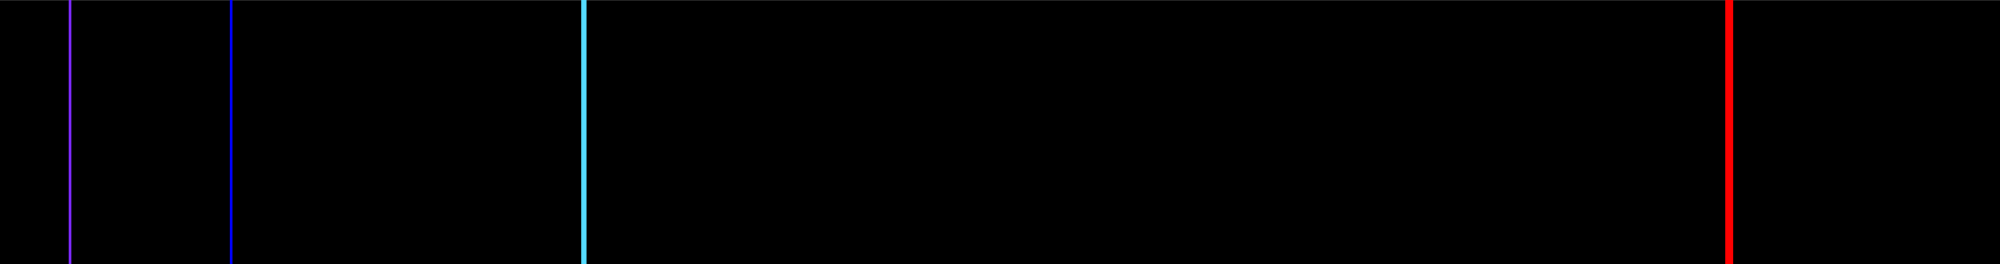
\includegraphics[scale=0.17]{HydrogenEmission.png}
\end{center}\caption{A small amount of hydrogen gas is place in a vacuum tube. A large voltage is applied which first separates \ce{H2} into atomic hydrogen, and then ionizes the atoms. When electrons and \ce{H+} recombine, light is emitted at discrete frequencies. A grating spectrometer splits the frequencies through different angles onto a dark wall. All visible transitions have $n_{f} = 2$ in \eqref{Rydberg}. From left to right, $n_{i} =6,5,4,3$. {\color{blue} Get the $n_{i}$'s under the emission lines!}}\label{HydrogenEmission}
\end{figure}
For this achievement, Bohr won a Nobel prize. More importantly, he was \href{http://www.youtube.com/watch?v=okJnQIjELY4#t=2m55s}{given} a house by the Carlsberg Brewing Company with a pipe into the house that let him drink as much beer as he wanted. 
Of course, not long thereafter he was willing to explain experimental data by throwing out the law of conservation of energy, so perhaps this was not such a good thing for Bohr. 
A nice refinement of the Bohr model was proposed in 1915 which stated that a periodic quantum system should be quantized according to 
\begin{align}\label{SommerfeldQuantization}
\oint p \, dq = nh, \qquad n \in \mathbb{N}.
\end{align}
The integral on the left is an intimidating object, but can be interpreted as representing the \emph{phase-space area} enclosed during one cycle of the motion (\figureref{PhaseSpace}).
\begin{figure}
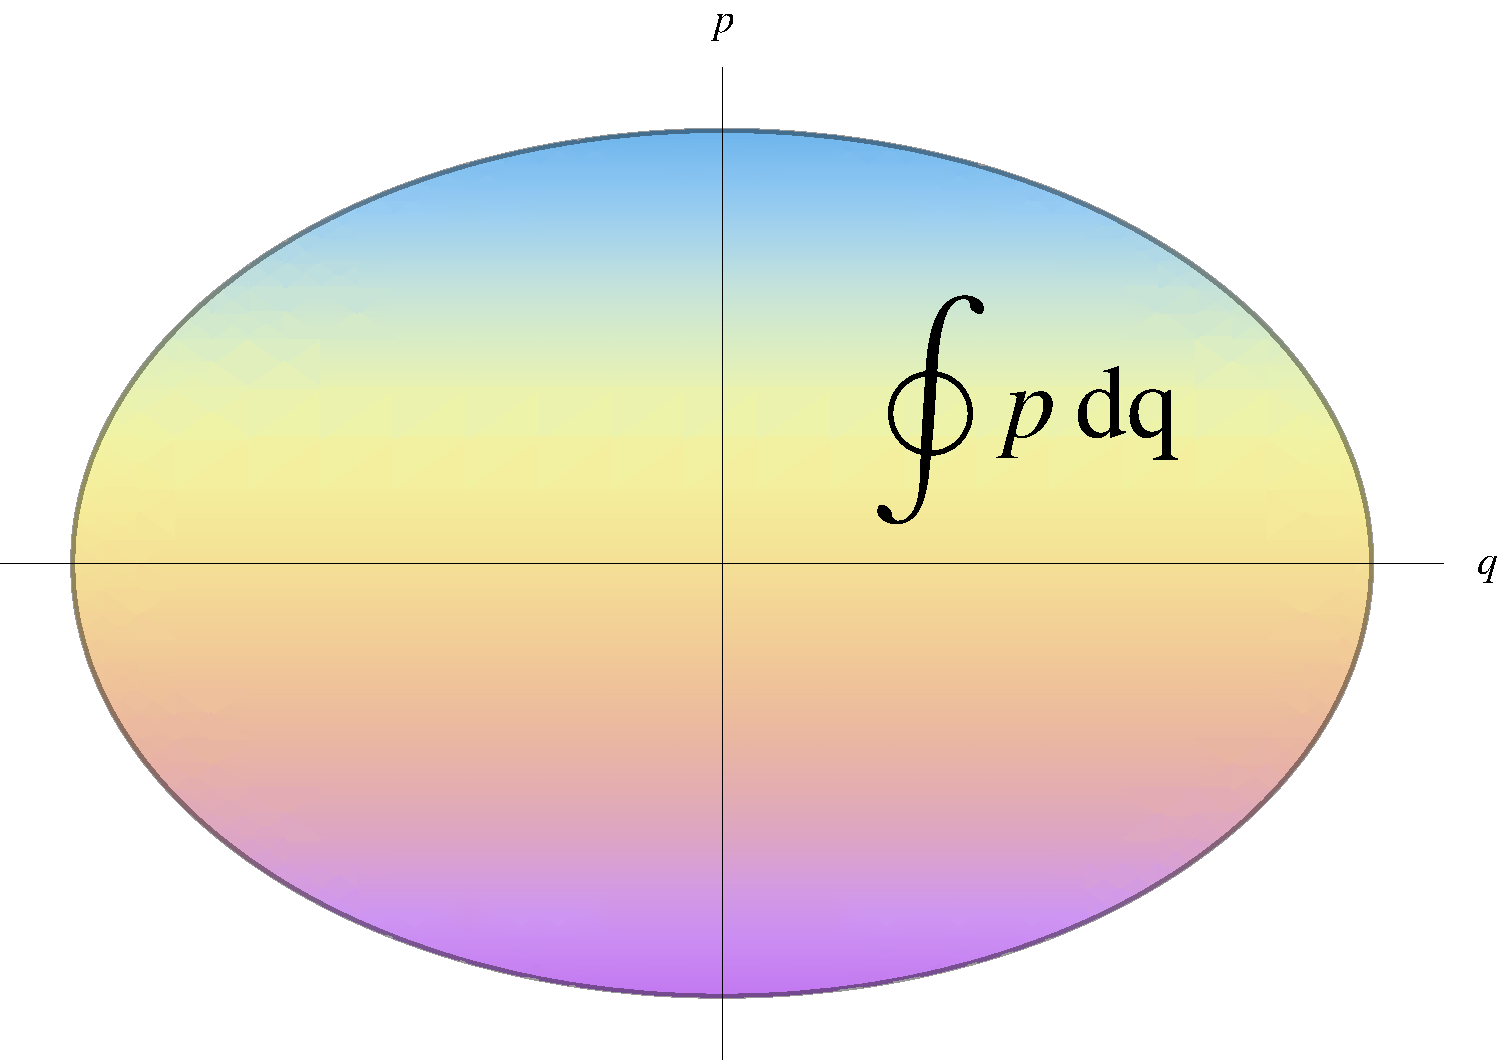
\includegraphics[scale=0.5]{SommerfeldWilson}
\caption{The term \emph{phase space} refers to all points $(q,p)$ in a $q$-$p$ coordinate plane. The contour integral \eqref{SommerfeldQuantization} can be intepreted as a \emph{phase-space area}.}\label{PhaseSpace}
\end{figure}


\begin{exercise}
Let $H = \frac{p^{2}}{2m} + \frac{1}{2}m\omega^{2}x^{2}$ be the harmonic oscillator Hamiltonian. Since $H$ does not depend explicitly on time, then $H=E$, the total energy. Hence $\frac{p^{2}}{2m} + \frac{1}{2}m\omega^{2}x^{2} = E$. 

\begin{enumerate}[(a)]

\item Write $\frac{p^{2}}{2m} + \frac{1}{2}m\omega^{2}x^{2} = E$ in the traditional form of an ellipse, i.e. write it as $\frac{x^{2}}{a^{2}} + \frac{y^{2}}{b^{2}} =1$. 

\item Isolate $p$ and calculate $\displaystyle\oint p \, dx$ over one period of the motion. 

\item\label{ptxt} Solve Hamilton's equations to obtain $p$ and $x$ as a function of time. 

\item Use $p(t)$ and $x(t)$ from \itemref{ptxt} to calculate $\displaystyle\oint p \,dq$ via $\displaystyle\int_{0}^{T}  p(t) \dot{x}(t) \, dt$ over one period of the motion. 

\item Use the area formula for an ellipse to calculate $\displaystyle\oint p\, dq$.

\item Using \eqref{SommerfeldQuantization}, what are the allowed energies of the harmonic oscillator? 

\end{enumerate}

\end{exercise}
In classical mechanics, we can place arbitrary quantities of energy into our harmonic oscillator, i.e., in $\frac{p^{2}}{2m} + \frac{1}{2}m\omega^{2}x^{2} = E$ we can adjust $E$ continuously. 
Since the phase space area goes as $\frac{2\pi E}{\omega}$, this allows us to expand the area of the enclosed phase space continuously. 
But within the Bohr-Sommerfeld model the phase space area is quantized according to $E = n\hbar \omega$, so that phase space area can only increase in discrete chuncks with area $2\pi \hbar$ (\figureref{Jump}). 
\begin{figure}
\includegraphics[scale=1]{SommerfeldWilsonExpansion}
\caption{The inner ellipse represents a state $(x_{1},p_{1})$. The energy cannot be increased continuously, but rather ``jumps'' to state $(x_{2},p_{2})$, represented in phase space by the outer ellipse. The area difference between these two states is given by $2\pi \hbar$.}\label{Jump}
\end{figure}



\subsection{Poisson Brackets}\index{Poisson brackets}

Suppose we have a system with $n$ degrees of freedom, and let $u$ and $v$ be any infinitely differentiable functions of the generalized momenta $\{p_{i}\}_{i=1}^{n}$ and $\{q_{i}\}_{i=1}^{n}$, and the time $t$. 
Then we can define the \emph{Poisson bracket} of $u$ and $v$ via
\begin{align*}
[u,v]:= \sum_{i=1}^{n} \frac{\partial u}{\partial q_{i}} \frac{\partial v}{\partial p_{i}} - \frac{\partial u}{\partial p_{i}} \frac{\partial v}{\partial q_{i}}.
\end{align*}
The Poisson brackets have innumerable mathematical properties that make them extremely entertaining, including:
\begin{itemize}
\item Bilinearity, 
\item Skew-symmetry, i.e., $[u,v] = -[v,u]$, and 
\item The Jacobi identity: $[u,[v,w]] + [v,[w,u]] + [w,[u,v]] = 0$. 
\end{itemize}
This means that the Poisson brackets are an example of a \emph{Lie bracket}, which endows the space of infinitely differentiable functions with the structure of a Lie algebra. 




\begin{exercise}
For a particle free to move in 3D space, compute the following Poisson brackets:
\begin{enumerate}[(a)]

\item $[x_{i},x_{j}]$ (where $x_{1} := x$, $x_{2} :=y$, $x_{3}:=z$).

\item $[p_{i}, p_{j}]$.

\item $[x_{i}, p_{j}]$. \emph{Answer:} $\delta_{ij}$.

\end{enumerate}
\end{exercise}

\begin{exercise}
Show that the Poisson bracket is bilinear. 
\end{exercise}

\begin{exercise}
Verify that the Poisson brackets bear the following analogy to the product rule:
\begin{align*}
\frac{d}{dx}(vw) &= \frac{dv}{dx}w + v \frac{dw}{dx}	\\
[u,vw] &= [u,v]w + v[u,w]
\end{align*}
For this reason, the map $[u, \cdot]$ is called a \emph{derivation}. 
\end{exercise}


\section{Waves}\index{waves}
 \subsection{Classical Wave Equation}\index{wave equation!classical}
 \subsection{Plane Waves}\index{plane waves}
 \subsection{Phase, Phase Velocity, and Dispersion Relations}\index{phase velocity}\index{dispersion relation}
 \subsection{Reflection, Transmission, and Attenuation}\index{reflection}\index{transmission}\index{attenuation}
 \subsection{Two-Wave Interference and Beating}\index{interference}\index{beating}
 \subsection{Wave Packet, Group Velocity, and the Uncertainty Principle}\index{wave packet}\index{group velocity}\index{uncertainty principle}
 \subsection{Maxwell's Equations}\index{Maxwell's equations}
 \subsection{AC Drude Conductivity}\index{Drude conductivity}
 \subsection{Propagation of an Electromagnetic Wave in a Medium}




\printindex
\printnomenclature
\end{document}